\documentclass[final,3p,times,authoryear]{elsarticle}

%% The amssymb package provides various useful mathematical symbols
\usepackage{amssymb}
\usepackage{amsmath}
\usepackage[colorlinks=true,linkcolor=blue,citecolor=blue,urlcolor=blue]{hyperref}
\usepackage[table]{xcolor}
\usepackage{booktabs}
\usepackage{multirow}
\usepackage{tikz}
\usetikzlibrary{positioning, arrows.meta, shapes.geometric}

\newcommand{\LreconC}{\mathcal{L}_{\text{recon,c}}}
\newcommand{\LreconG}{\mathcal{L}_{\text{recon,g}}}
\newcommand{\LKL}{\mathcal{L}_{\text{KL}}}
\newcommand{\LCox}{\mathcal{L}_{\text{Cox}}}
\newcommand{\Lcross}{\mathcal{L}_{\text{cross}}}
\newcommand{\Ltotal}{\mathcal{L}_{\text{total}}}

\renewcommand{\topfraction}{0.95}
\renewcommand{\dbltopfraction}{0.95}
\renewcommand{\bottomfraction}{0.95}
\renewcommand{\textfraction}{0.05}
\renewcommand{\floatpagefraction}{0.95}
\renewcommand{\dblfloatpagefraction}{0.95}

\let\oldthebibliography\thebibliography
\renewcommand{\thebibliography}[1]{%
  \oldthebibliography{#1}%
  \setlength{\itemsep}{0pt}%
  \setlength{\parskip}{0pt}%
}

\journal{Machine Learning with Applications}
\begin{document}

\begin{frontmatter}

\title{Survival Integration via Generative Multi-omics Alignment (SIGMA)}

\author[1,2]{Azman Nads\corref{cor1}}
\ead{azmannads@msutawi-tawi.edu.ph}
\cortext[cor1]{Corresponding author}

\author[3]{Alkajim Aradais}
\author[4]{Amina Nasirin}
\author[3]{Anuarisa Aradais}

\affiliation[1]{organization={Informatics and Data Science Program, Graduate School of Advanced Science and Engineering},
            addressline={1-4-1 Kagamiyama}, 
            city={739-8527 Higashihiroshima},
            state={Hiroshima},
            country={Japan}}

\affiliation[2]{organization={Department of Statistics, College of Mathematical Sciences, Mindanao State University Tawi-Tawi College of Technology and Oceanography},
            addressline={Sanga-Sanga},
            city={Bongao},
            postcode={7500},
            state={Tawi-Tawi},
            country={Philippines}}

\affiliation[3]{organization={Department of Mathematics, College of Mathematical Sciences, Mindanao State University Tawi-Tawi College of Technology and Oceanography},
            addressline={Sanga-Sanga},
            city={Bongao},
            postcode={7500},
            state={Tawi-Tawi},
            country={Philippines}}

\affiliation[4]{organization={Office of the Vice Chancellor for Academic Affairs, Mindanao State University Tawi-Tawi College of Technology and Oceanography},
            addressline={Sanga-Sanga},
            city={Bongao},
            postcode={7500},
            state={Tawi-Tawi},
            country={Philippines}}

\begin{abstract}
The integration of heterogeneous clinical and genomic data improves survival prediction in oncology. However, biological datasets frequently suffer from Missing Not At Random (MNAR) missingness, wherein the probability of missingness depends on the unobserved value itself through threshold-interaction mechanisms. Prior multi-omics survival models assume missing data occurs at random and do not explicitly model MNAR mechanisms across heterogeneous modalities. This paper presents Survival Integration via Generative Multi-omics Alignment (SIGMA), a multimodal variational autoencoder designed to address threshold-interaction MNAR conditions. SIGMA uses modality-specific encoders and cross-modal latent alignment to construct a shared representation optimized jointly for feature reconstruction, cross-modal alignment, and survival prediction. Three fusion strategies were evaluated: Early Fusion (EF), Cross-Modal Attention (CMA), and Product of Experts (PoE), using the METABRIC breast cancer cohort ($N=1{,}979$) under systematically simulated MNAR conditions. Under severe missingness, SIGMA CMA achieved the lowest clinical RMSE among multimodal deep learning methods ($0.703 \pm 0.034$) and competitive genomic RMSE ($0.908 \pm 0.015$). SIGMA EF achieved a downstream random survival forest C-index of $0.643 \pm 0.018$ under severe missingness, comparable to MICE ($0.648 \pm 0.014$) and missForest ($0.644 \pm 0.014$). SIGMA CMA achieved the highest PAM50 molecular subtype classification accuracy among deep learning methods ($0.648 \pm 0.035$). PoE exhibited instability consistent with posterior collapse under joint missingness conditions. An ablation study confirmed that explicit missingness mask concatenation was the most critical architectural factor, with its removal increasing clinical RMSE from $0.720$ to $0.797$. Classical iterative imputation methods remained competitive for biological subtype classification, while SIGMA showed a distinct advantage in cross-modal genomic reconstruction, with CMA achieving a C2G RMSE of $1.049 \pm 0.007$ under severe missingness.
\end{abstract}

\begin{keyword}
Missing Not At Random \sep Multimodal survival analysis \sep Variational autoencoder \sep Genomic imputation \sep METABRIC \sep Cross-modal alignment \sep Latent fusion
\end{keyword}

\end{frontmatter}

\section{Introduction}
\label{sec:intro}

Accurate prediction of patient survival in oncology depends on the ability to integrate multiple sources of clinical and molecular information. A single data type rarely captures the full picture of disease progression: clinical variables reflect patient history and treatment response, while genomic profiles reveal tumor biology and molecular subtype, and each carries prognostic information the other does not \citep{curtis2012genomic}. Combining both is therefore central to precision oncology, but doing so exposes a problem that single-modality models can avoid: missing data in each modality rarely occurs by chance.

Electronic health records and genomic sequencing datasets commonly contain missing values that arise from unobserved clinical decisions, sequencing failures, or patient-specific factors such as age or disease severity. This missingness is frequently missing not at random (MNAR), meaning the probability that a value is missing depends on the value itself, rather than on other observed variables \citep{rubin1976inference,little2019statistical}. This is not a minor technical detail. Standard imputation methods, including multiple imputation by chained equations (MICE) and missForest, assume missing at random (MAR) or missing completely at random (MCAR) conditions \citep{buuren2011mice,stekhoven2012missforest}, and produce biased estimates when applied to data where missingness carries information about the underlying value. In a clinical setting, this bias can distort survival risk estimates in exactly the patients for whom accurate prediction matters most, those with more severe or advanced disease, since severity is often what drives both the missingness and the outcome.

\citet{mnarsvae} addressed this problem for unimodal clinical data with a variational autoencoder (VAE) trained jointly with a Cox proportional hazards loss under threshold-interaction MNAR conditions, an age-stratified missingness mechanism in which the probability of a value being missing depends on whether a patient's age crosses a defined threshold. The model achieved a concordance index (C-index) of 0.693 with random survival forests (RSF) and 0.693 with XGBoost on the MIMIC-IV sepsis cohort under severe missingness. This result confirms that explicit MNAR modeling yields a measurable and growing benefit as missingness severity increases, and that the benefit is concentrated precisely in the harder, more clinically relevant regime. This model, however, processes only a single data modality and cannot incorporate genomic profiles, which limits its applicability to oncology settings where multi-omics integration is often necessary for a complete risk assessment.

Multimodal variational autoencoders for multi-omics survival prediction exist \citep{chang2025myevae,chen2026moriskvae}, along with cross-modal attention fusion \citep{li2023mavae}, product-of-experts fusion \citep{wu2018multimodal}, and cross-modal contrastive alignment \citep{li2025cpathomic,rajaram2024dacmva}. These methods establish that multi-omics fusion architectures for survival prediction are both feasible and effective. None of them, however, explicitly model threshold-dependent informative missingness across modalities. They either assume complete data or treat missing modalities as random dropout at the modality level, which fails to capture the value-dependent missingness patterns frequently observed in real clinical and genomic data; the threshold-interaction MNAR mechanism used here is designed to better approximate such patterns, though it remains a controlled simulation. This leaves a specific and unaddressed gap: to our knowledge, no existing multi-omics survival model accounts for informative, threshold-dependent missingness occurring jointly across heterogeneous data types.

This gap has direct clinical significance. If missingness in either clinical or genomic data is informative rather than random, and existing multi-omics models do not account for this, then survival risk estimates produced by these models may be systematically biased in ways that are difficult to detect without an explicit missingness-aware framework. Closing this gap requires extending threshold-interaction MNAR modeling from the unimodal setting to a multimodal one, without discarding the demonstrated benefits of cross-modal fusion.

This paper presents Survival Integration via Generative Multi-omics Alignment (SIGMA), which extends the threshold-interaction MNAR mechanism of \citet{mnarsvae} to joint clinical and genomic modalities within a survival-aware generative framework. The objective of this work is threefold: to model informative, threshold-dependent MNAR missingness jointly across clinical and genomic data within a single generative framework; to evaluate whether a shared latent representation aligned across modalities preserves survival-relevant and biologically meaningful structure under this missingness condition; and to characterize how established multimodal fusion strategies, specifically early fusion, cross-modal attention, and product of experts, perform under threshold-interaction MNAR conditions rather than under the completeness or random-dropout assumptions used in prior evaluations. SIGMA does not propose a new fusion architecture; its contribution is the explicit modeling of joint MNAR missingness within an established multimodal survival framework, a mechanism absent from all prior multi-omics survival methods reviewed in Section \ref{sec:related_work}.

\section{Related Work}
\label{sec:related_work}

\subsection{Missing data under MNAR conditions}
\citet{rubin1976inference} established the taxonomy of MCAR, MAR, and MNAR mechanisms; \citet{little2019statistical} extended this framework for statistical inference under incomplete data. MICE \citep{buuren2011mice} and missForest \citep{stekhoven2012missforest} both assume MAR conditions and produce biased imputations when this assumption does not hold. Generative approaches including GAIN \citep{yoon2018gain}, MIDA \citep{gondara2018mida}, and MIWAE \citep{mattei2019miwae} improved imputation accuracy on tabular data but were not designed for informative, value-dependent missingness patterns, and none of these methods incorporate a survival objective.

\subsection{Survival analysis on complete data}
The Cox proportional hazards model \citep{cox1972regression} remains the standard framework for time-to-event prediction under proportional hazards assumptions. RSF \citep{ishwaran2008random} extended this to a non-parametric ensemble approach. Deep learning approaches include DeepSurv \citep{katzman2018deepsurv}, which combined a Cox partial likelihood with a feedforward network, and DeepHit \citep{lee2018deephit}, which modeled the full survival distribution directly and handled competing risks. All of these methods assume complete input data.

\subsection{Multimodal fusion architectures}
Product-of-experts fusion for multimodal variational autoencoders \citep{wu2018multimodal} combined unimodal posteriors under a precision-weighted Gaussian assumption, originally applied to weakly supervised multimodal learning outside the clinical domain. Cross-modal attention \citep{vaswani2017attention} was adapted for unaligned multimodal sequences \citep{tsai2019multimodal} and for clinical risk prediction through MAVAE \citep{li2023mavae}, which applied multi-head attention across modalities for cancer risk prediction but assumed complete multi-omics input.

\subsection{Multi-omics survival models}
MyeVAE \citep{chang2025myevae} combined a multimodal variational autoencoder with a Cox loss for risk profiling in multiple myeloma, establishing the base architecture pattern of modality-specific encoders feeding a shared survival network. However, MyeVAE relies exclusively on simple latent concatenation without cross-modal alignment mechanisms. MO-RiskVAE \citep{chen2026moriskvae} extended this architecture through latent regularization on the MMRF CoMMpass dataset but did not compare fusion strategies, did not use contrastive alignment, and did not model MNAR missingness. CPathomic \citep{li2025cpathomic} combined cross-modal contrastive learning with attention for cancer survival prediction on pathology and genomic data, but assumed complete modalities. DACMVA \citep{rajaram2024dacmva} addressed missing modalities in cancer survival prediction through data augmentation, but operated under missing completely at random modality dropout rather than informative, threshold-dependent missingness.

Across this body of work, missingness is either absent from the modeling assumptions or treated as random dropout at the modality level. None of these methods model threshold-dependent MNAR missingness within individual modalities, nor jointly across heterogeneous modalities, within a survival-aware framework. SIGMA addresses this gap directly.

\section{Methods}
\label{sec:methods}

Figure~\ref{fig:framework} illustrates the SIGMA pipeline for integrating clinical and genomic data under informative missingness. The framework covers data simulation, multimodal imputation, and downstream evaluation across survival prediction and biological validity tasks.

\begin{figure*}[!t]
\centering
\resizebox{\textwidth}{!}{%
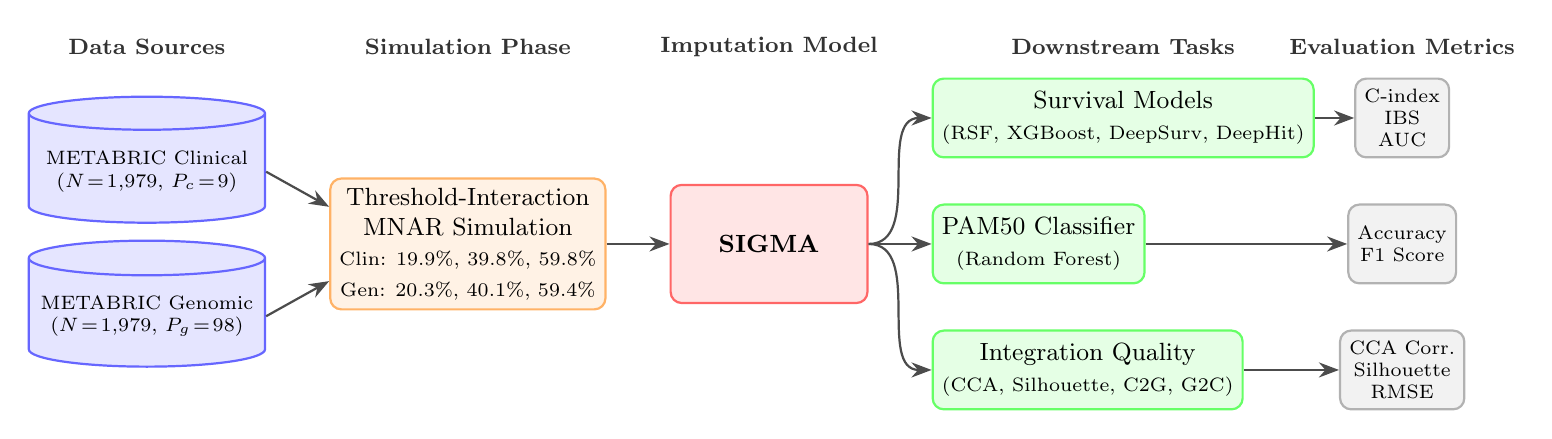
\begin{tikzpicture}[
    >={Stealth[scale=1.1]},
    box/.style={rectangle, draw, rounded corners, minimum height=1cm, align=center, text opacity=1, font=\small, thick},
    datanode/.style={cylinder, shape border rotate=90, aspect=0.15, draw, minimum height=1.6cm, minimum width=3cm, align=center, font=\scriptsize, thick, fill=blue!10, draw=blue!60},
    simnode/.style={box, fill=orange!10, draw=orange!60},
    modelnode/.style={box, fill=red!10, draw=red!60, minimum width=2.5cm, minimum height=1.5cm},
    evalnode/.style={box, fill=green!10, draw=green!60},
    metricnode/.style={box, fill=gray!10, draw=gray!60, font=\scriptsize},
    grouplabel/.style={font=\footnotesize\bfseries, align=center, text=black!80},
    arr/.style={->, thick, draw=black!70}
]

% Data sources
\node[datanode] (data_c) {METABRIC Clinical \\ ($N\!=\!1{,}979$, $P_c\!=\!9$)};
\node[datanode, below=0.2cm of data_c] (data_g) {METABRIC Genomic \\ ($N\!=\!1{,}979$, $P_g\!=\!98$)};

% MNAR simulation
\path (data_c.east) -- (data_g.east) coordinate[midway] (mid_east);
\node[simnode, right=0.8cm of mid_east] (mnar) {Threshold-Interaction \\ MNAR Simulation \\ \scriptsize{Clin: 19.9\%, 39.8\%, 59.8\%} \\ \scriptsize{Gen: 20.3\%, 40.1\%, 59.4\%}};

\draw[arr] (data_c.east) -- (mnar.165);
\draw[arr] (data_g.east) -- (mnar.195);

% SIGMA model
\node[modelnode, right=0.8cm of mnar] (sigma) {\textbf{SIGMA}};

\draw[arr] (mnar.east) -- (sigma.west);

% Downstream
\node[evalnode, right=0.8cm of sigma, yshift=1.6cm] (surv_model) {Survival Models \\ \scriptsize{(RSF, XGBoost, DeepSurv, DeepHit)}};
\node[evalnode, right=0.8cm of sigma] (pam_model) {PAM50 Classifier \\ \scriptsize{(Random Forest)}};
\node[evalnode, right=0.8cm of sigma, yshift=-1.6cm] (integ_model) {Integration Quality \\ \scriptsize{(CCA, Silhouette, C2G, G2C)}};

\draw[arr] (sigma.east) to[out=0, in=180] (surv_model.west);
\draw[arr] (sigma.east) -- (pam_model.west);
\draw[arr] (sigma.east) to[out=0, in=180] (integ_model.west);

% Metrics
\node[metricnode, right=0.5cm of surv_model] (surv_metric) {C-index \\ IBS \\ AUC};
\node[metricnode] at (surv_metric |- pam_model) (pam_metric) {Accuracy \\ F1 Score};
\node[metricnode] at (surv_metric |- integ_model) (integ_metric) {CCA Corr. \\ Silhouette \\ RMSE};

\draw[arr] (surv_model.east) -- (surv_metric.west);
\draw[arr] (pam_model.east) -- (pam_metric.west);
\draw[arr] (integ_model.east) -- (integ_metric.west);

% Group Labels
\node[grouplabel, above=0.4cm of data_c] (label_data) {Data Sources};
\node[grouplabel] at (mnar |- label_data) {Simulation Phase};
\node[grouplabel] at (sigma |- label_data) {Imputation Model};
\node[grouplabel] at (surv_model |- label_data) {Downstream Tasks};
\node[grouplabel] at (surv_metric |- label_data) {Evaluation Metrics};

\end{tikzpicture}%
}

\caption{Methodological framework of the study, illustrating the data pipeline from threshold-interaction MNAR simulation to downstream survival prediction and biological validation.}
\label{fig:framework}
\end{figure*}

\subsection{Problem Formulation}
The dataset contains $N$ samples, where each sample $i$ has clinical features $\mathbf{x}_{c,i} \in \mathbb{R}^{P_c}$ and genomic features $\mathbf{x}_{g,i} \in \mathbb{R}^{P_g}$. The survival outcome for each sample is $\mathcal{O}_i = (T_i, E_i)$. The variable $T_i = \min(t_i, c_i)$ is the observed time, where $t_i$ is the true event time and $c_i$ is the censoring time. The event indicator $E_i \in \{0, 1\}$ equals 1 if $t_i \leq c_i$. The missingness masks are $\mathbf{M}_{c,i} \in \{0,1\}^{P_c}$ and $\mathbf{M}_{g,i} \in \{0,1\}^{P_g}$, where $M_{c,ij} = 1$ indicates feature $j$ of sample $i$ is missing in the clinical modality, and equivalently for the genomic modality. The observed index sets are $\Omega_c = \{(i,j) : M_{c,ij} = 0\}$ and $\Omega_g = \{(i,j) : M_{g,ij} = 0\}$. The clinical encoder receives $[\mathbf{x}_{c,i}, \mathbf{M}_{c,i}] \in \mathbb{R}^{2P_c}$ and the genomic encoder receives $[\mathbf{x}_{g,i}, \mathbf{M}_{g,i}] \in \mathbb{R}^{2P_g}$, following the mask-concatenation input convention of the base MNAR-SVAE model. SIGMA jointly imputes missing values in both modalities and predicts the survival hazard from the shared latent representation.

\subsection{MNAR-SVAE}
The base model for this study is MNAR-SVAE \citep{mnarsvae}, which addresses threshold-interaction MNAR missingness in unimodal clinical survival data. Threshold-interaction MNAR is defined as a missingness mechanism in which the probability that a feature value is missing depends on whether another observed variable, specifically patient age, crosses a defined threshold. This mechanism is clinically motivated and captures non-linear, age-stratified missingness patterns absent from standard linear MNAR simulation frameworks.

The encoder receives the concatenated input $[\mathbf{X}, \mathbf{M}] \in \mathbb{R}^{2P}$, where $\mathbf{X} \in \mathbb{R}^{N \times P}$ is the feature matrix and $\mathbf{M} \in \{0,1\}^{N \times P}$ is the binary missingness mask with $M_{ij} = 1$ indicating that feature $j$ of sample $i$ is missing. The encoder maps this input to the parameters $\mu$ and $\log \sigma^2$ of a Gaussian distribution. The latent vector is sampled via the reparameterization trick: $\mathbf{z} = \mu + \sigma \odot \epsilon$, where $\epsilon \sim \mathcal{N}(\mathbf{0}, \mathbf{I})$.

The decoder reconstructs $\hat{\mathbf{X}}$ from $\mathbf{z}$. The reconstruction loss $\mathcal{L}_{\text{recon}}$ is a masked mean squared error computed only over the observed index set $\Omega = \{(i,j) : M_{ij} = 0\}$, so the model is not penalized for its reconstruction of missing values during training.

A survival network $f_\psi$ predicts the log-hazard $\eta = f_\psi(\mathbf{z})$, optimized via the Cox partial likelihood \citep{cox1972regression} $\mathcal{L}_{\text{Cox}}$. The composite loss is:
\begin{equation}
\mathcal{L}_{\text{total}} = \mathcal{L}_{\text{recon}} + \beta \cdot \mathcal{L}_{\text{KL}} + \gamma \cdot \mathcal{L}_{\text{Cox}}
\end{equation}
where $\mathcal{L}_{\text{KL}}$ is the Kullback-Leibler divergence between the posterior and $\mathcal{N}(\mathbf{0}, \mathbf{I})$. Survival outcomes $\mathcal{O} = (T, E)$ enter only through $\mathcal{L}_{\text{Cox}}$ during training. At inference, the encoder receives only $[\mathbf{X}, \mathbf{M}]$.

MNAR-SVAE was validated on METABRIC ($N = 1{,}904$) and MIMIC-IV sepsis ($N = 32{,}065$) \citep{johnson2023mimic} under light, moderate, and severe threshold-interaction MNAR conditions. On MIMIC-IV under severe missingness, MNAR-SVAE achieved a C-index of $0.693$ with random survival forests \citep{ishwaran2008random} and $0.693$ with XGBoost. MNAR-SVAE processes only unimodal clinical data, which motivates the multimodal extension in SIGMA.

\subsection{Architecture}

Figure~\ref{fig:architecture} details the multimodal variational autoencoder network architecture. Modality-specific encoders map clinical and genomic inputs to unimodal latent spaces, which are aligned via contrastive loss and fused into a shared representation for reconstruction and survival prediction.
\begin{figure*}[!t]
\centering
\resizebox{\textwidth}{!}{%
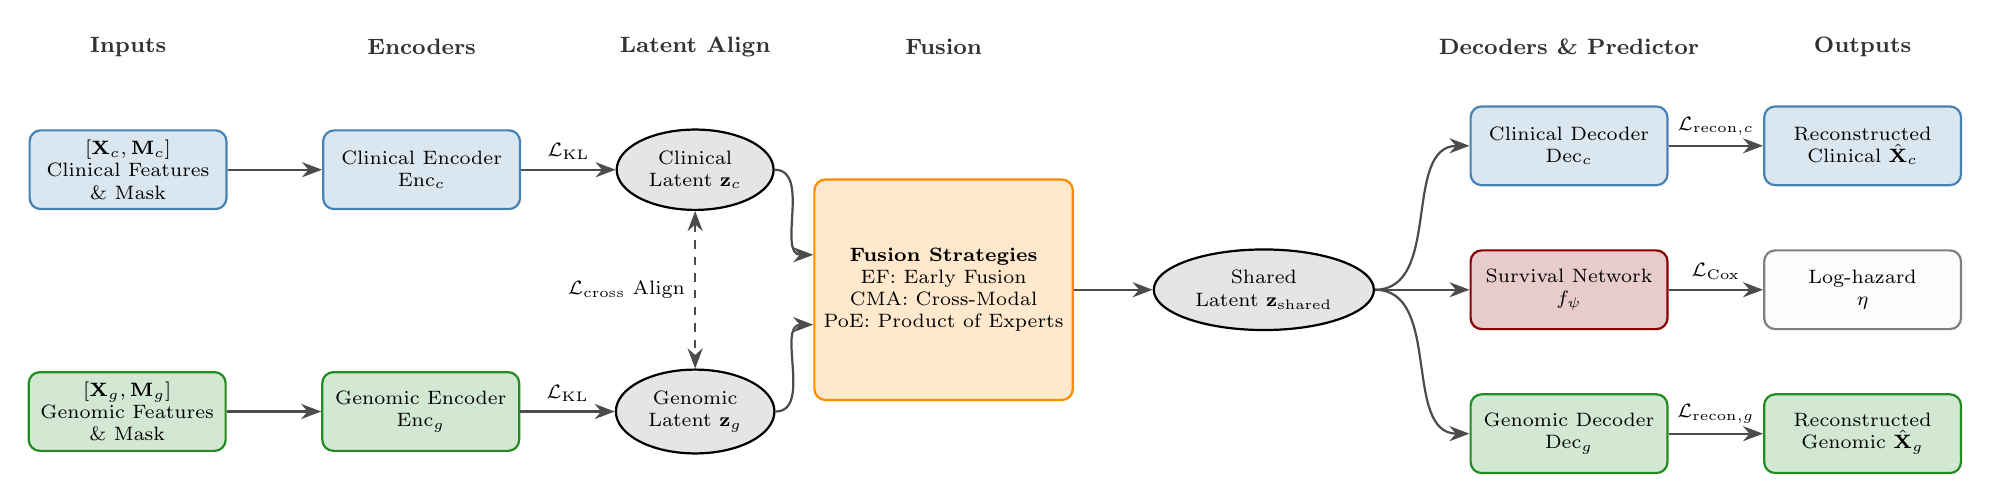
\begin{tikzpicture}[
    >={Stealth[scale=1.1]},
    box/.style={rectangle, draw, rounded corners, minimum width=2.5cm, minimum height=1cm, align=center, fill opacity=0.2, text opacity=1, font=\scriptsize, thick},
    circ/.style={ellipse, draw, minimum width=1.5cm, minimum height=1cm, align=center, fill=gray!20, font=\scriptsize, thick},
    grouplabel/.style={font=\footnotesize\bfseries, align=center, text=black!80},
    arr/.style={->, thick, draw=black!70},
    biarr/.style={<->, thick, dashed, draw=black!70}
]

% Define colors
\definecolor{clincol}{RGB}{70, 130, 180} % steel blue
\definecolor{gencol}{RGB}{34, 139, 34}   % forest green
\definecolor{fuscol}{RGB}{255, 140, 0}   % dark orange
\definecolor{survcol}{RGB}{139, 0, 0}    % dark red

% Latent Layer (Center point for symmetry)
\node[circ] (zc) {Clinical \\ Latent $\mathbf{z}_c$};
\node[circ, below=2cm of zc] (zg) {Genomic \\ Latent $\mathbf{z}_g$};
\path (zc) -- (zg) coordinate[midway] (midz);

\draw[biarr] (zc) -- node[left, font=\scriptsize] {$\mathcal{L}_{\text{cross}}$ Align} (zg);

% Encoder Layer
\node[box, draw=clincol, fill=clincol, left=1.2cm of zc] (encc) {Clinical Encoder \\ $\text{Enc}_c$};
\node[box, draw=gencol, fill=gencol, left=1.2cm of zg] (encg) {Genomic Encoder \\ $\text{Enc}_g$};

\draw[arr] (encc) -- node[above, font=\scriptsize] {$\mathcal{L}_{\text{KL}}$} (zc);
\draw[arr] (encg) -- node[above, font=\scriptsize] {$\mathcal{L}_{\text{KL}}$} (zg);

% Input Layer
\node[box, draw=clincol, fill=clincol, left=1.2cm of encc] (inc) {$[\mathbf{X}_c, \mathbf{M}_c]$ \\ Clinical Features \\ \& Mask};
\node[box, draw=gencol, fill=gencol, left=1.2cm of encg] (ing) {$[\mathbf{X}_g, \mathbf{M}_g]$ \\ Genomic Features \\ \& Mask};

\draw[arr] (inc) -- (encc);
\draw[arr] (ing) -- (encg);

% Fusion Layer
\node[box, draw=fuscol, fill=fuscol, right=1.5cm of midz, minimum height=2.8cm] (fusion) {\textbf{Fusion Strategies} \\ EF: Early Fusion \\ CMA: Cross-Modal \\ PoE: Product of Experts};
\node[circ, right=1cm of fusion] (zshared) {Shared \\ Latent $\mathbf{z}_{\text{shared}}$};

\draw[arr] (zc.east) to[out=0, in=180] (fusion.165);
\draw[arr] (zg.east) to[out=0, in=180] (fusion.195);
\draw[arr] (fusion) -- (zshared);

% Decoder & Survival Layer
\node[box, draw=survcol, fill=survcol, right=1.2cm of zshared] (surv) {Survival Network \\ $f_\psi$};
\node[box, draw=clincol, fill=clincol, above=0.8cm of surv] (decc) {Clinical Decoder \\ $\text{Dec}_c$};
\node[box, draw=gencol, fill=gencol, below=0.8cm of surv] (decg) {Genomic Decoder \\ $\text{Dec}_g$};

\draw[arr] (zshared) to[out=0, in=180] (decc.west);
\draw[arr] (zshared) to[out=0, in=180] (decg.west);
\draw[arr] (zshared) -- (surv.west);

% Output Layer
\node[box, draw=clincol, fill=clincol, right=1.2cm of decc] (outc) {Reconstructed \\ Clinical $\hat{\mathbf{X}}_c$};
\node[box, draw=gray, fill=gray!10] (eta) at (surv -| outc) {Log-hazard \\ $\eta$};
\node[box, draw=gencol, fill=gencol] (outg) at (decg -| outc) {Reconstructed \\ Genomic $\hat{\mathbf{X}}_g$};

\draw[arr] (decc) -- node[above, font=\scriptsize] {$\mathcal{L}_{\text{recon},c}$} (outc);
\draw[arr] (decg) -- node[above, font=\scriptsize] {$\mathcal{L}_{\text{recon},g}$} (outg);
\draw[arr] (surv) -- node[above, font=\scriptsize] {$\mathcal{L}_{\text{Cox}}$} (eta);

% Group Labels
\node[grouplabel, above=0.8cm of inc] (label_in) {Inputs};
\node[grouplabel] at (encc |- label_in) {Encoders};
\node[grouplabel] at (zc |- label_in) {Latent Align};
\node[grouplabel] at (fusion |- label_in) {Fusion};
\node[grouplabel] at (decc |- label_in) {Decoders \& Predictor};
\node[grouplabel] at (outc |- label_in) {Outputs};

\end{tikzpicture}%
}

\caption{The SIGMA model architecture. Modality-specific encoders map clinical and genomic features to latent spaces, which are aligned via contrastive loss. A fusion module aggregates them into a shared representation, from which decoders reconstruct the inputs and a Cox proportional hazards network predicts survival outcomes. Each labeled loss component and input block was systematically evaluated in the ablation study (Section~\ref{sec:ablation}).}
\label{fig:architecture}
\end{figure*}
SIGMA uses separate encoders for each modality, following the modality-specific encoder pattern of \citet{chang2025myevae}. Clinical and genomic data differ in dimensionality, noise distribution, and missingness pattern, and separate encoders allow each modality to learn its own feature-level representation before any cross-modal interaction occurs. Each encoder receives the concatenated feature vector and missingness mask as input, following the mask-concatenation convention of \citet{mnarsvae}. Under threshold-interaction MNAR, the pattern of absent values carries information about the underlying unobserved values, and encoding the mask alongside the features allows the encoder to learn which absence patterns are informative rather than treating all missing entries as equivalent.

Each encoder outputs the parameters of a Gaussian distribution: $\mu_c$ and $\log \sigma_c^2$ for the clinical encoder, and $\mu_g$ and $\log \sigma_g^2$ for the genomic encoder. The unimodal latent representations are sampled via the reparameterization trick of \citet{kingma2014auto}: $\mathbf{z}_c = \mu_c + \sigma_c \odot \epsilon$ and $\mathbf{z}_g = \mu_g + \sigma_g \odot \epsilon$, where $\epsilon \sim \mathcal{N}(\mathbf{0}, \mathbf{I})$.

A fusion module combines $\mathbf{z}_c$ and $\mathbf{z}_g$ into $\mathbf{z}_{\text{shared}}$; the specific fusion strategies are described in the following subsection. Two modality-specific decoders, $\text{Dec}_c$ and $\text{Dec}_g$, reconstruct the clinical and genomic inputs from $\mathbf{z}_{\text{shared}}$ rather than from the unimodal latents. Forcing both decoders to reconstruct from the shared representation requires the fusion module to retain modality-specific information, and it is intended to encourage the shared space to capture sufficient structure for imputation in either modality.

A survival network $f_\psi$ operates on $\mathbf{z}_{\text{shared}}$ to predict the log-hazard $\eta$, which is passed to the Cox survival loss during training. The survival network operates on $\mathbf{z}_{\text{shared}}$ rather than on the unimodal latents because the shared representation is the only space that has been jointly regularized across both modalities, and survival prediction from a jointly aligned space is expected to be more reliable than prediction from modality-specific spaces that have not been brought into correspondence.

\subsection{Fusion Strategies}
SIGMA evaluates three fusion strategies to compute $\mathbf{z}_{\text{shared}}$, each adopted from established multimodal variational autoencoder literature rather than proposed as new, citing \citet{chang2025myevae}, \citet{li2023mavae}, and \citet{wu2018multimodal}. Prior comparisons of these strategies assumed complete data or random modality dropout, and it is not known how each strategy behaves when missingness is informative and threshold-dependent. The three strategies differ in how they handle differential information quality across modalities when one modality is more heavily affected by missingness than the other.

\textbf{Early Fusion (EF).} Early Fusion (EF) is the simplest strategy, concatenating $\mathbf{z}_c$ and $\mathbf{z}_g$ and projecting linearly:
\begin{equation}
\mathbf{z}_{\text{shared}} = \mathbf{W}_{\text{EF}}[\mathbf{z}_c ; \mathbf{z}_g] + \mathbf{b}_{\text{EF}}
\label{eq:ef}
\end{equation}
Concatenation treats both modalities symmetrically regardless of their relative completeness, which may be a poor assumption when one modality is substantially more missing than the other under threshold-interaction MNAR.

\textbf{Cross-Modal Attention (CMA).} Cross-Modal Attention (CMA) follows \citet{vaswani2017attention} and \citet{tsai2019multimodal}, applied to clinical risk prediction by \citet{li2023mavae} under completeness assumptions:
\begin{equation}
\begin{split}
\mathbf{z}_{c,\text{att}} &= \text{Attention}(Q=\mathbf{z}_c,\ K=\mathbf{z}_g,\ V=\mathbf{z}_g), \\
\mathbf{z}_{g,\text{att}} &= \text{Attention}(Q=\mathbf{z}_g,\ K=\mathbf{z}_c,\ V=\mathbf{z}_c)
\end{split}
\label{eq:cma-att}
\end{equation}
\begin{equation}
\mathbf{z}_{\text{shared}} = \mathbf{W}_{\text{CMA}}[\mathbf{z}_{c,\text{att}} ; \mathbf{z}_{g,\text{att}}] + \mathbf{b}_{\text{CMA}}
\label{eq:cma-proj}
\end{equation}
Each modality queries the other using attention, allowing the clinical representation to selectively weight genomic features it finds relevant and vice versa. When one modality is heavily missing, its latent representation carries less information, and attention is expected to allow the more complete modality to dominate the shared representation adaptively rather than contributing equally.

\textbf{Product of Experts (PoE).} Product of Experts (PoE) follows \citet{wu2018multimodal}:
\begin{equation}
p(\mathbf{z} \mid \mathbf{x}_c, \mathbf{x}_g) \propto p(\mathbf{z} \mid \mathbf{x}_c) \cdot p(\mathbf{z} \mid \mathbf{x}_g)
\label{eq:poe-prop}
\end{equation}
\begin{equation}
\mu_{\text{shared}} = \sigma_{\text{shared}}^2 \left( \frac{\mu_c}{\sigma_c^2} + \frac{\mu_g}{\sigma_g^2} \right), \qquad \sigma_{\text{shared}}^2 = \left( \frac{1}{\sigma_c^2} + \frac{1}{\sigma_g^2} \right)^{-1}
\label{eq:poe-params}
\end{equation}
All operations in Equations~\ref{eq:poe-prop} and~\ref{eq:poe-params} are applied element-wise across the $d$-dimensional latent space.
The joint posterior is dominated by whichever modality has lower variance, meaning higher certainty. When a modality is heavily affected by threshold-interaction MNAR missingness, the encoder for that modality is expected to produce higher-variance posterior estimates, and the precision weighting should theoretically reduce its influence on the shared representation without requiring explicit missingness-aware logic.

\subsection{Composite Loss}
SIGMA is trained end-to-end with five loss components that serve distinct but complementary roles. Reconstruction losses push the latent space to preserve raw feature variation so that imputation is accurate, while the Cox survival loss pushes the latent space to preserve prognostically relevant variation, and the $\lambda_{\text{Cox}}$ hyperparameter governs this trade-off. This joint training ensures imputation is survival-aware rather than treating imputation and prediction as independent steps, which is the key distinction from pipelines that apply imputation and survival modeling separately.

The clinical and genomic reconstruction losses, $\LreconC$ and $\LreconG$, compute masked mean squared error over $\Omega_c$ and $\Omega_g$ respectively, following \citet{mnarsvae}. Computing the loss only over observed entries means the model is not penalized for its reconstruction of missing values during training, which is necessary under MNAR because the missing values are not missing at random and their true values are unobserved.

The Kullback-Leibler divergence $\LKL$ is defined as the KL divergence between the shared posterior and $\mathcal{N}(\mathbf{0}, \mathbf{I})$, following \citet{kingma2014auto}. It regularizes $\mathbf{z}_{\text{shared}}$ to prevent posterior collapse and ensures the shared space remains well-structured for both imputation and survival prediction. In the product of experts variant, unregularized modality posteriors with very high variance dominate the precision weighting incorrectly, so KL regularization is especially important for this fusion strategy.

The survival component applies the Cox partial likelihood \citep{cox1972regression}:
\begin{equation}
\LCox = -\frac{1}{N_{E=1}} \sum_{i : E_i=1} \left( \eta_i - \log \sum_{j : T_j \geq T_i} \exp(\eta_j) \right)
\label{eq:cox}
\end{equation}
where $E_i$ denotes the event indicator and $T_i$ the observed time for patient $i$, and $N_{E=1} = \sum_{i=1}^N E_i$ is the total number of observed events. Without $\LCox$, the shared latent space is optimized only for reconstruction and alignment, and the resulting imputations may be statistically accurate in terms of RMSE but fail to preserve the survival-relevant structure that distinguishes high-risk from low-risk patients.

A cross-modal contrastive loss $\Lcross$ aligns $\mathbf{z}_c$ and $\mathbf{z}_g$ using the InfoNCE estimator, following the contrastive alignment approach applied to cancer survival prediction by \citet{li2025cpathomic}. Here $\mathbf{z}_{c,i}$ and $\mathbf{z}_{g,i}$ denote the clinical and genomic latent vectors for sample $i$, with $\mathbf{z}_{g,j}$ denoting the genomic latent vector for a distinct sample $j$:
\begin{equation}
\Lcross = -\frac{1}{N} \sum_{i=1}^N \log \frac{\exp(\text{sim}(\mathbf{z}_{c,i}, \mathbf{z}_{g,i}) / \kappa)}{\sum_{j=1}^N \exp(\text{sim}(\mathbf{z}_{c,i}, \mathbf{z}_{g,j}) / \kappa)}
\label{eq:infonce}
\end{equation}
where $\text{sim}(\cdot,\cdot)$ denotes cosine similarity, $\kappa$ denotes the temperature hyperparameter, and $N$ denotes the mini-batch size ($B = 128$) rather than the full cohort size; contrastive negative pairs are sampled within each training batch. Same-patient clinical-genomic pairs are treated as positives and cross-patient pairs as negatives, so minimizing $\Lcross$ pulls the clinical and genomic latent vectors for the same patient together while pushing apart those from different patients. Without $\Lcross$, $\mathbf{z}_c$ and $\mathbf{z}_g$ can occupy different regions of the latent space with no correspondence, which breaks cross-modal imputation because the clinical encoder cannot infer genomic structure and vice versa.

The total objective combines these terms:
\begin{equation}
\Ltotal = \LreconC + \LreconG + \lambda_{\text{KL}} \cdot \LKL + \lambda_{\text{Cox}} \cdot \LCox + \lambda_{\text{cross}} \cdot \Lcross
\label{eq:total}
\end{equation}
The $\lambda_{\text{KL}}$ hyperparameter controls the strength of KL regularization, $\lambda_{\text{Cox}}$ controls the weight of the survival objective relative to reconstruction, and $\lambda_{\text{cross}}$ controls the strength of cross-modal alignment. These were selected via Bayesian optimization over the ranges specified in the Implementation Details subsection.

\subsection{Datasets}
Two breast cancer cohorts were used for model training and evaluation: the Molecular Taxonomy of Breast Cancer International Consortium (METABRIC) \citep{curtis2012genomic} and The Cancer Genome Atlas (TCGA) PanCanAtlas Breast Invasive Carcinoma (BRCA) cohort. The METABRIC dataset was filtered to the Nature 2012 primary cohort. The final METABRIC dataset contained $N = 1{,}979$ patients with complete multi-omics data, of whom $1{,}143$ ($57.76\%$) experienced the event of interest (death due to disease). 

The clinical feature set ($P_c = 9$) consisted of age at diagnosis, chemotherapy, hormone therapy, radiotherapy, estrogen receptor (ER) status, human epidermal growth factor receptor 2 (HER2) status, progesterone receptor (PR) status, MKI67 expression, and EGFR expression. MKI67 and EGFR were extracted from the z-scored microarray expression matrix rather than the clinical file, consistent with standard METABRIC practice, as these genes served as proxy biomarkers in this dataset. Continuous clinical features (age at diagnosis, MKI67, and EGFR) were z-score standardized. Binary categorical features (chemotherapy, hormone therapy, radiotherapy, ER status, HER2 status, and PR status) were encoded as $0$ and $1$. 

The genomic feature set ($P_g = 98$) comprised $49$ PAM50 (a 50-gene expression panel used for breast cancer molecular subtyping) gene expression features and $49$ gene-level discrete copy number alteration features. The expression features were extracted from the z-scored microarray data, and the copy number alterations were GISTIC (Genomic Identification of Significant Targets in Cancer)-derived discrete values. The CTSL2 gene was absent from the expression matrices of both datasets and was excluded; the remaining $49$ PAM50 genes were used. The survival outcome consisted of overall survival time in months and an event indicator, encoded as $0$ for living and $1$ for deceased. Patients with missing or zero overall survival time were excluded.

The TCGA PanCanAtlas BRCA cohort was accessed via cBioPortal and serves as an external validation set for the genomic modalities. The final TCGA dataset contained $N = 1{,}055$ patients after excluding $13$ patients with missing or zero overall survival time and intersecting the clinical records with complete expression and copy number alteration data. The TCGA genomic feature set contained the same $49$ PAM50 gene expression features and $49$ copy number alteration features. TCGA does not contain chemotherapy, hormone therapy, PR status, or HER2 status in the standard PanCanAtlas clinical files; clinical feature imputation is therefore evaluated on METABRIC only. TCGA is used exclusively to evaluate genomic imputation quality, survival prediction, and biological pathway preservation. The PAM50 molecular subtype (LumA, LumB, Her2, Basal, Normal) was available in the clinical records and is used for silhouette score evaluation of latent space cluster quality.


\subsection{Missingness Simulation}

The threshold-interaction MNAR mechanism is defined for the SIGMA architecture. For modality $m \in \{c, g\}$ and feature $j$, the probability that feature $j$ of sample $i$ is missing is
\begin{equation}
P(M_{m,ij} = 1 \mid a_i, x_{m,ij}) = \text{sigmoid}\!\left(\alpha_m \cdot \mathbf{1}[a_i > \tau] \cdot |x_{m,ij}| + \beta_m\right)
\label{eq:mnar}
\end{equation}
where $\text{sigmoid}(\cdot)$ is the logistic sigmoid function, $a_i$ is patient age at diagnosis, $\tau = 0.056$ is the median age of the METABRIC cohort (z-score standardized), $\alpha_m$ controls the interaction strength for modality $m$, and $\beta_m$ controls the baseline missingness rate. This mechanism makes missingness informative: feature values that are large in magnitude and occur in older patients are more likely to be missing, which violates the MAR assumption. Each feature $j$ drives its own missingness via its magnitude $|x_{m,ij}|$ interacting with the age threshold indicator. MKI67 and ESR1 are representative examples of features with high self-masking probability under this mechanism due to their biological association with patient age in the METABRIC cohort \citep{qing2022molecular}.

Parameters $\alpha_m$ and $\beta_m$ were calibrated separately for each modality and each severity level to achieve target missingness proportions of $p_{\text{miss}} \in \{0.20, 0.40, 0.60\}$, corresponding to light, moderate, and severe missingness respectively. Calibration searched over $\alpha_m \in \{0.5, 1.0, 2.0, \ldots, 10.0\}$ and $\beta_m \in \{-5.0, -4.5, \ldots, 0.0\}$, selecting the combination whose achieved missingness rate, averaged over ten random seeds, was closest to the target. The calibrated parameters are presented in Table \ref{tab:mnar_params}.

\begin{table}[t]
\caption{Calibrated threshold-interaction MNAR parameters for each modality and severity level. Target and achieved missingness proportions are reported. Parameters were calibrated on the METABRIC cohort ($N = 1{,}979$) using ten random seeds.}
\label{tab:mnar_params}
\centering
\rowcolors{2}{gray!10}{white}
\begin{tabular}{llcccc}
\toprule
Modality & Severity & Target $p_{\text{miss}}$ & $\alpha_m$ & $\beta_m$ & Achieved $p_{\text{miss}}$ \\
\midrule
Clinical & Light & 0.20 & 6.0 & -4.5 & 0.1991 \\
 & Moderate & 0.40 & 6.0 & -1.5 & 0.3980 \\
 & Severe & 0.60 & 2.0 & 0.0 & 0.5978 \\
Genomic & Light & 0.20 & 4.0 & -3.5 & 0.2031 \\
 & Moderate & 0.40 & 10.0 & -3.0 & 0.4014 \\
 & Severe & 0.60 & 4.0 & -0.5 & 0.5936 \\
\bottomrule
\end{tabular}
\end{table}

Two simulation conditions were evaluated. Under independent missingness, the mechanism was applied to each modality separately using independently calibrated parameters, producing modality-specific missingness patterns. Under joint missingness, a single shared age threshold $\tau$ was applied across both modalities simultaneously with the same calibrated parameters, producing correlated missingness patterns across clinical and genomic features. A fully observed subset of METABRIC patients was identified prior to simulation by retaining only patients with no missing values in the raw clinical and genomic feature matrices; this subset served as the ground truth for imputation quality evaluation. The same mechanism was applied to the TCGA genomic modality using the parameters calibrated on METABRIC, with $\tau$ set to the median age of the TCGA cohort.

The genomic moderate condition required $\alpha_g = 10.0$, the maximum value in the search grid, to achieve the target proportion of 0.40, while the clinical modality required only $\alpha_c = 6.0$ for the same target. This difference indicates that the ESR1-age interaction in the METABRIC expression data is weaker than the MKI67-age interaction, requiring a stronger scaling parameter to produce equivalent missingness rates. Under severe missingness, the clinical modality calibrated to $\beta_c = 0.0$, meaning the baseline probability of missingness in the absence of the age-interaction term is $\text{sigmoid}(0) = 0.50$; this reflects the high overall missingness burden at the severe level and is relevant when interpreting modality-specific imputation performance in the Results section.

\subsection{Baselines}

MNAR-SVAE \citep{mnarsvae} is a unimodal generative model that handles threshold-interaction MNAR conditions through a joint survival-aware architecture. It assumes missingness is MNAR and models it explicitly by incorporating a binary missingness mask. In this study, MNAR-SVAE was applied exclusively to the clinical modality with no genomic input. This method lacks a genomic encoder and cross-modal fusion capabilities, serving as the direct predecessor to SIGMA and representing the strongest unimodal baseline. In this study, MNARSVAE hyperparameters were selected using the same Optuna Bayesian optimization protocol and composite validation objective as SIGMA, ensuring a fair comparison.

MyeVAE \citep{chang2025myevae} serves as a multimodal deep learning baseline. The architecture consists of two modality-specific VAE encoders that map clinical and genomic inputs to independent latent representations, which are concatenated into a shared latent vector. Modality-specific decoders reconstruct the original inputs from the shared representation, and a Cox proportional hazards network predicts the log-hazard. MyeVAE does not employ cross-modal attention or contrastive alignment. Because MyeVAE lacks a native missingness handling mechanism, missing values were filled using training-set imputation prior to model input under all missingness conditions.

The standard VAE \citep{kingma2014auto} is a VAE trained without a survival objective. It assumes missingness is MAR. In this study, the standard VAE was applied to the clinical modality using the identical encoder and decoder architecture as MNAR-SVAE, but the survival objective weight was set to $\lambda_{\text{Cox}} = 0$. This baseline lacks the Cox partial likelihood loss, testing whether the survival-aware objective improves imputation and prediction over a standard generative model.

MICE \citep{buuren2011mice} estimates missing values sequentially using conditional models for each feature. It assumes missingness is MAR. MICE was applied independently to the clinical and genomic modalities. MICE lacks a joint multimodal representation, a survival objective, and explicit MNAR modeling.

missForest \citep{stekhoven2012missforest} is a non-parametric alternative to MICE that imputes missing values using random forests. It assumes missingness is MAR. In this study, missForest was applied independently to each modality. Like MICE, it lacks a joint multimodal representation, a survival objective, and explicit MNAR modeling.

GAIN \citep{yoon2018gain} adapts the generative adversarial framework for missing data imputation. It assumes missingness is MAR. GAIN was applied independently to each modality. This baseline lacks a survival objective, explicit MNAR modeling, and cross-modal fusion capabilities.

Multiple imputation using denoising autoencoders (MIDA) \citep{gondara2018mida} reconstructs missing values by learning low-dimensional representations of corrupted input. It assumes missingness is MAR. MIDA was applied independently to each modality. It lacks a survival objective, explicit MNAR modeling, and cross-modal fusion capabilities.

The SIGMA clinical-only ablation is a restricted version of the full architecture that retains the clinical encoder and decoder but removes the genomic components and the fusion module. It assumes missingness is MNAR. This ablation was trained exclusively on clinical data under threshold-interaction MNAR conditions. It lacks the genomic modality, testing the contribution of the genomic modality to the imputation and prediction tasks.

The SIGMA genomic-only ablation retains the genomic encoder and decoder while removing the clinical components and the fusion module. It assumes missingness is MNAR. This ablation was trained exclusively on genomic expression data under threshold-interaction MNAR conditions. It lacks the clinical modality, testing the contribution of the clinical modality to the imputation and prediction tasks.

\subsection{Evaluation Metrics}

Within-modality imputation quality is evaluated using root mean square error (RMSE) and mean absolute error (MAE), computed per modality over artificially masked values only. The ground truth was the fully observed subset identified prior to missingness simulation. RMSE and MAE are formally defined for modality $m \in \{c, g\}$ as:
\begin{equation}
\text{RMSE}_m = \sqrt{\frac{1}{|\Omega_m^{\text{mask}}|} \sum_{(i,j) \in \Omega_m^{\text{mask}}} (\hat{x}_{m,ij} - x_{m,ij})^2}
\label{eq:rmse}
\end{equation}
\begin{equation}
\text{MAE}_m = \frac{1}{|\Omega_m^{\text{mask}}|} \sum_{(i,j) \in \Omega_m^{\text{mask}}} |\hat{x}_{m,ij} - x_{m,ij}|
\label{eq:mae}
\end{equation}
where $\hat{x}_{m,ij}$ is the imputed value, $x_{m,ij}$ is the true value, and $\Omega_m^{\text{mask}} = \{(i,j) : M_{m,ij} = 1\}$ is the set of artificially masked indices.

Cross-modality imputation quality is evaluated using RMSE and MAE computed when one modality's encoder is used to infer features of the other modality. Two directions were evaluated: the clinical encoder predicting genomic features, and the genomic encoder predicting clinical features. This evaluates whether the shared latent space enables cross-modal inference under threshold-interaction MNAR conditions.

Survival prediction performance is evaluated using the C-index, integrated Brier score (IBS), and time-dependent area under the receiver operating characteristic curve (AUC) at 1, 3, and 5 years. These time points reflect standard clinical benchmarks in breast cancer prognosis: 1-year AUC captures early mortality risk relevant to aggressive subtypes, 3-year AUC reflects medium-term prognosis commonly reported in adjuvant therapy trials, and 5-year overall survival is the primary benchmark in breast cancer outcomes research \citep{sparano2018adjuvant}. The C-index is formally defined as the proportion of all comparable patient pairs for which the model correctly orders survival times. Downstream survival models, specifically RSF \citep{ishwaran2008random}, XGBoost, DeepSurv \citep{katzman2018deepsurv}, and DeepHit \citep{lee2018deephit}, were trained on the imputed data produced by each method and evaluated on held-out test sets under 5-fold cross-validation. Formal significance testing was not performed since the minimum achievable p-value under a two-sided Wilcoxon signed-rank test with $n=5$ paired observations is $p=0.0625$, which exceeds the standard $\alpha=0.05$ threshold even before multiple comparison correction \citep{conover1999practical}.



Integration quality is evaluated using two metrics. First, canonical correlation analysis (CCA) between $\mathbf{z}_c$ and $\mathbf{z}_g$ measures the linear alignment between the clinical and genomic latent representations; a higher CCA correlation indicates better cross-modal alignment in the shared space. Second, the silhouette score is computed on $\mathbf{z}_{\text{shared}}$ using known PAM50 molecular subtypes (LumA, LumB, Her2, Basal, Normal) as cluster labels; a higher silhouette score indicates that the shared latent space preserves biologically meaningful subtype structure.

Biological validity is evaluated by assessing whether imputed PAM50 gene expression preserves molecular subtype structure. A random forest classifier is trained on the ground truth PAM50 expression values using the known PAM50 molecular subtypes (LumA, LumB, Her2, Basal, Normal) as labels, then applied to imputed expression values to predict subtypes. Classification accuracy and macro-averaged F1 score are reported. This evaluation follows the standard practice for biological validation in METABRIC-based multi-omics studies \citep{curtis2012genomic} and is evaluated at the severe missingness level only, since preservation of subtype structure under high missingness represents the most stringent test of biological validity.



\subsection{Implementation Details}

SIGMA was implemented in PyTorch. All experiments were run under 5-fold cross-validation with stratified splits preserving the event rate across folds. Per fold, the training set contained approximately $1{,}424$ patients, the validation set $159$ patients, and the test set $396$ patients, with an event rate of approximately $0.578$ in each split.

Each encoder consists of two fully connected layers with ReLU activations, mapping to a latent dimension $d$. Each decoder mirrors the encoder structure. The survival network $f_\psi$ is a two-layer feedforward network with a single scalar output representing the log-hazard $\eta$. The cross-modal attention in the CMA fusion strategy uses a single attention head.

Hyperparameters were selected via Bayesian optimization using Optuna \citep{akiba2019optuna} with 50 trials per fold, evaluated on the fold-specific validation set under a nested cross-validation scheme. Each trial trained the model for a maximum of 50 epochs and was evaluated using a composite objective that balances imputation quality and survival discrimination: $\text{objective} = \mathcal{L}_{\text{recon,val}} - \lambda_{\text{surv}} \cdot \text{C-index}_{\text{val}}$, where $\lambda_{\text{surv}} = 2.0$ was set to emphasize survival discrimination while maintaining reconstruction quality, following multi-task loss balancing principles \citep{kendall2018multitask, chapfuwa2020survival}. The best hyperparameters identified for each fold were used for that fold's full training run of up to 200 epochs with early stopping. The search ranges were $d \in \{32, 64, 128\}$ for the latent dimension, $\lambda_{\text{KL}} \in [0.01, 2.0]$ for the KL weight, $\lambda_{\text{Cox}} \in [0.1, 5.0]$ for the Cox weight, $\lambda_{\text{cross}} \in [0.1, 1.0]$ for the cross-modal alignment weight, $\kappa \in [0.05, 0.5]$ for the InfoNCE temperature, and $\eta_{\text{lr}} \in [10^{-4}, 10^{-2}]$ for the learning rate. All continuous hyperparameters were sampled from log-uniform distributions using the TPE sampler \citep{akiba2019optuna}. The model was trained using the Adam optimizer with a batch size of 128 and a maximum of 200 epochs. Early stopping was applied with a patience of 20 epochs based on the composite validation objective.

MICE and missForest were applied using their standard implementations with default hyperparameters. GAIN and MIDA were implemented following their original papers \citep{yoon2018gain, gondara2018mida} with hyperparameters set to the values reported in those papers. MyeVAE was subjected to the exact same Optuna hyperparameter tuning protocol, search space, and composite objective function as SIGMA to ensure rigorous scientific fairness. Downstream survival models (RSF, XGBoost, DeepSurv, DeepHit) were trained on the completed datasets produced by each imputation method using their default hyperparameters unless otherwise specified. All methods were evaluated under identical cross-validation splits.

All random seeds were fixed at 42 for final mask generation and model initialization. Code and preprocessed data will be made available upon acceptance.



\section{Results}
\label{sec:results}

\subsection{Imputation Quality}

\begin{table*}[!t]
\centering
\rowcolors{2}{gray!10}{white}
\caption{RMSE for genomic expression imputation across all methods and severity levels (independent condition). Mean absolute error (MAE) results are provided in Table~\ref{tab:supp_mae_g}.}
\label{tab:imputation_g}
\begin{tabular}{lccc}
\toprule
Method & Light (20.31\%) & Moderate (40.14\%) & Severe (59.36\%) \\
\midrule
SIGMA EF & $1.145 \pm 0.023$ & $1.017 \pm 0.019$ & $0.929 \pm 0.013$ \\
SIGMA CMA & $1.162 \pm 0.015$ & $1.040 \pm 0.010$ & $0.908 \pm 0.015$ \\
SIGMA PoE & $1.222 \pm 0.022$ & $1.045 \pm 0.012$ & $0.917 \pm 0.014$ \\
MyeVAE & $1.225 \pm 0.019$ & $1.040 \pm 0.018$ & $0.945 \pm 0.010$ \\
MICE & $1.122 \pm 0.025$ & $\mathbf{0.991 \pm 0.014}$ & $\mathbf{0.887 \pm 0.010}$ \\
missForest & $\mathbf{1.065 \pm 0.019}$ & $1.012 \pm 0.013$ & $\mathbf{0.887 \pm 0.014}$ \\
GAIN & $1.257 \pm 0.018$ & $1.072 \pm 0.015$ & $0.996 \pm 0.008$ \\
MIDA & $1.201 \pm 0.022$ & $1.026 \pm 0.016$ & $0.918 \pm 0.010$ \\
\bottomrule
\end{tabular}

\vspace{1ex}
\footnotesize{Note: Values are reported as mean $\pm$ standard deviation (SD). Best values are highlighted in bold. RMSE: Root Mean Square Error; EF: Early Fusion; CMA: Cross-modal Attention; PoE: Product of Experts; MICE: Multiple Imputation by Chained Equations.}
\end{table*}

\begin{table*}[!t]
\centering
\rowcolors{2}{gray!10}{white}
\caption{RMSE for clinical feature imputation across all methods and severity levels (independent condition). Mean absolute error (MAE) results are provided in Table~\ref{tab:supp_mae_c}.}
\label{tab:imputation_c}
\begin{tabular}{lccc}
\toprule
Method & Light (19.91\%) & Moderate (39.80\%) & Severe (59.78\%) \\
\midrule
SIGMA EF & $0.881 \pm 0.054$ & $0.821 \pm 0.035$ & $0.720 \pm 0.033$ \\
SIGMA CMA & $0.853 \pm 0.047$ & $0.873 \pm 0.032$ & $0.703 \pm 0.034$ \\
SIGMA PoE & $0.869 \pm 0.024$ & $0.862 \pm 0.017$ & $0.673 \pm 0.032$ \\
MyeVAE & $0.786 \pm 0.047$ & $0.772 \pm 0.025$ & $0.639 \pm 0.021$ \\
MICE & $\mathbf{0.659 \pm 0.042}$ & $\mathbf{0.634 \pm 0.028}$ & $\mathbf{0.547 \pm 0.007}$ \\
missForest & $0.682 \pm 0.056$ & $0.687 \pm 0.022$ & $0.573 \pm 0.028$ \\
GAIN & $0.810 \pm 0.030$ & $0.783 \pm 0.018$ & $0.679 \pm 0.018$ \\
MIDA & $0.851 \pm 0.039$ & $0.786 \pm 0.028$ & $0.675 \pm 0.021$ \\
StandardVAE & $0.783 \pm 0.042$ & $0.714 \pm 0.027$ & $0.668 \pm 0.024$ \\
MNARSVAE & $0.882 \pm 0.061$ & $0.857 \pm 0.021$ & $0.731 \pm 0.016$ \\
\bottomrule
\end{tabular}

\vspace{1ex}
\footnotesize{Note: Values are reported as mean $\pm$ standard deviation (SD). Best values are highlighted in bold. RMSE: Root Mean Square Error; EF: Early Fusion; CMA: Cross-modal Attention; PoE: Product of Experts; MICE: Multiple Imputation by Chained Equations; VAE: Variational Autoencoder; MNAR: Missing Not At Random.}
\end{table*}

Table~\ref{tab:imputation_g} and Table~\ref{tab:imputation_c} report imputation performance for genomic expression and clinical features, respectively. Under severe threshold-interaction missingness, MICE and missForest achieved the lowest genomic RMSE at $0.887 \pm 0.010$ and $0.887 \pm 0.014$, respectively. Among multimodal deep learning methods, SIGMA CMA achieved the lowest genomic RMSE at $0.908 \pm 0.015$, followed by SIGMA EF at $0.929 \pm 0.013$ and SIGMA PoE at $0.917 \pm 0.014$. For clinical imputation under severe missingness, SIGMA PoE achieved the lowest RMSE among all evaluated methods at $0.673 \pm 0.032$, followed by SIGMA CMA at $0.703 \pm 0.034$ and MyeVAE at $0.639 \pm 0.021$. MICE achieved a clinical RMSE of $0.547 \pm 0.007$ under severe missingness. Figure~\ref{fig:rmse_severity} plots genomic imputation RMSE across severity levels for all evaluated methods.

\begin{figure*}[!t]
\centering
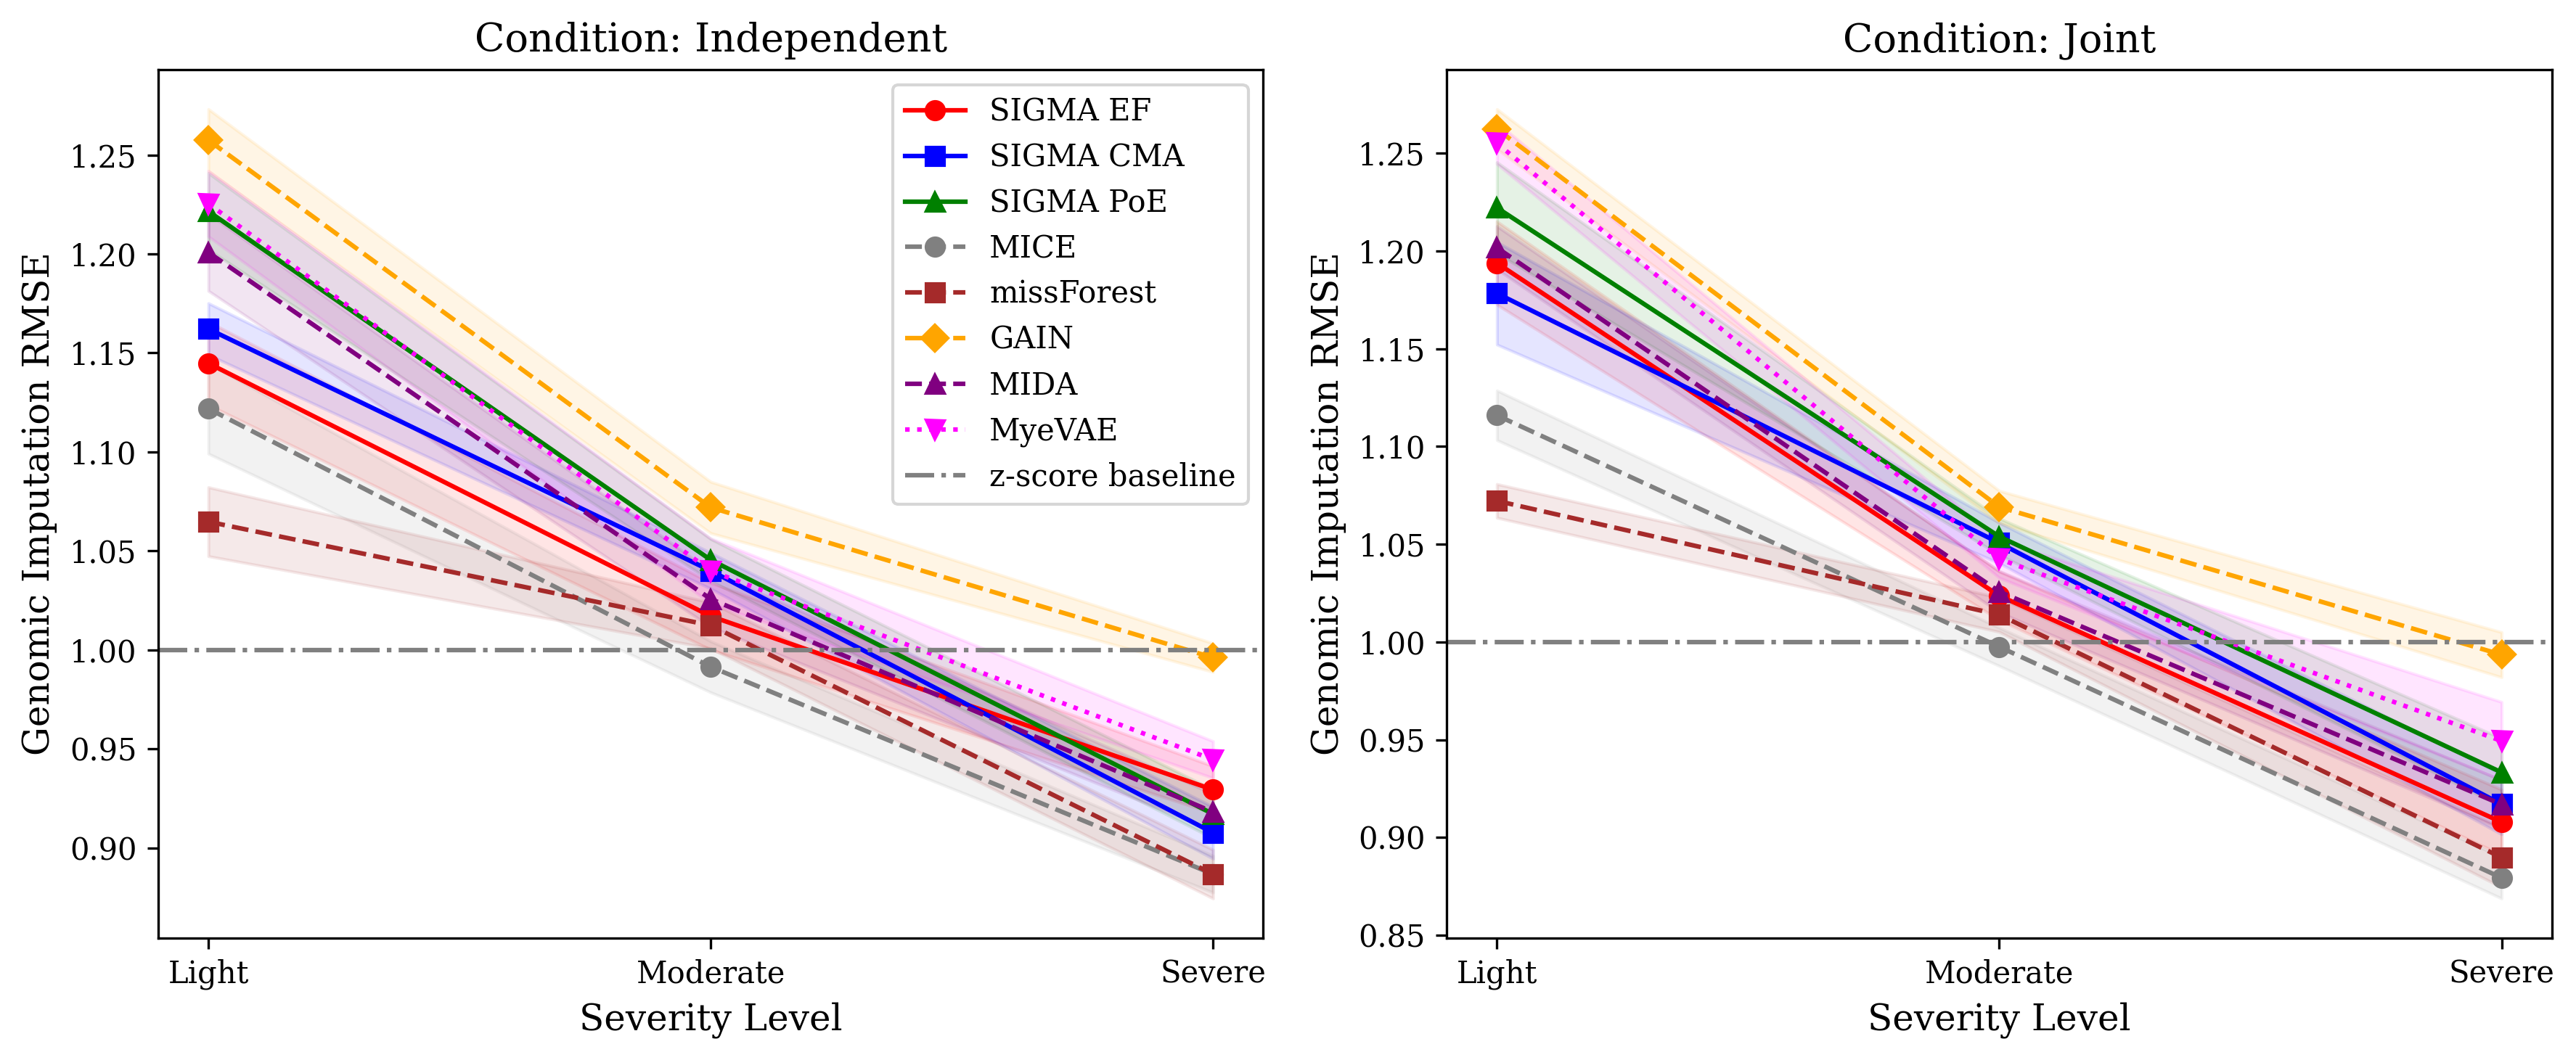
\includegraphics[width=\textwidth]{rmse_by_severity.png}
\caption{Genomic imputation RMSE across missingness severity levels for all evaluated methods under independent (left) and joint (right) simulation conditions. Lower values indicate better imputation quality. Error bands represent one standard deviation across five cross-validation folds.}
\label{fig:rmse_severity}
\end{figure*}

\subsection{Ablation Study}
\label{sec:ablation}

Table~\ref{tab:ablation} reports imputation and downstream evaluation metrics for five ablation variants of SIGMA Early Fusion under severe independent missingness.

\begin{table*}[!t]
\centering
\rowcolors{2}{gray!10}{white}
\caption{Ablation study results for SIGMA Early Fusion under severe independent missingness.}
\label{tab:ablation}
\resizebox{\textwidth}{!}{%
\begin{tabular}{lcccccc}
\toprule
Metric & Full SIGMA EF & w/o $\mathcal{L}_{\text{cross}}$ & w/o $\mathcal{L}_{\text{Cox}}$ & w/o Mask Input & Clinical-only & Genomic-only \\
\midrule
$\text{RMSE}_c$ & $0.720 \pm 0.033$ & $0.707 \pm 0.036$ & $0.699 \pm 0.031$ & $0.797 \pm 0.024$ & $0.704 \pm 0.021$ & --- \\
$\text{RMSE}_g$ & $0.929 \pm 0.013$ & $0.909 \pm 0.014$ & $0.909 \pm 0.013$ & $0.917 \pm 0.011$ & --- & $0.934 \pm 0.013$ \\
C-index RSF & $0.643 \pm 0.018$ & $0.638 \pm 0.007$ & $0.627 \pm 0.011$ & $0.635 \pm 0.013$ & $0.612 \pm 0.016$ & $0.598 \pm 0.017$ \\
PAM50 Acc & $0.628 \pm 0.027$ & $0.664 \pm 0.038$ & $0.671 \pm 0.036$ & $0.646 \pm 0.032$ & --- & $0.588 \pm 0.029$ \\
\bottomrule
\end{tabular}%
}

\vspace{1ex}
\footnotesize{Note: Values are reported as mean $\pm$ standard deviation (SD) across 5 cross-validation folds. `---' indicates the modality or task is not applicable for the variant. $\text{RMSE}_c$: clinical RMSE; $\text{RMSE}_g$: genomic expression RMSE; C-index RSF: concordance index from random survival forest; PAM50 Acc: PAM50 molecular subtype classification accuracy; EF: Early Fusion.}
\end{table*}

Removing the mask input $[\mathbf{x}, \mathbf{M}]$ from the encoder produced the largest degradation across all metrics, increasing clinical RMSE from $0.720$ to $0.797$ and reducing PAM50 accuracy from $0.628$ to $0.646$. Explicit missingness encoding was therefore the most critical architectural component under threshold-interaction MNAR conditions. Removing the contrastive alignment loss $\mathcal{L}_{\text{cross}}$ did not degrade imputation RMSE ($0.707$ vs $0.720$), which placed its contribution in latent space organization rather than direct reconstruction. Removing Cox supervision $\mathcal{L}_{\text{Cox}}$ reduced the downstream C-index from $0.643$ to $0.627$ without improving imputation RMSE substantially ($0.699$ vs $0.720$), confirming that survival-guided optimization shaped the latent space for discrimination rather than reconstruction. The clinical-only variant ($\text{RMSE}_c = 0.704 \pm 0.021$, C-index $= 0.612 \pm 0.016$) and the genomic-only variant ($\text{RMSE}_g = 0.934 \pm 0.013$, C-index $= 0.598 \pm 0.017$) both degraded relative to the full bimodal model, with the genomic-only variant showing the steepest C-index drop, confirming that clinical features drove survival discrimination in the METABRIC cohort.



\subsection{Survival Prediction}

\begin{table*}[!t]
\centering
\rowcolors{2}{gray!10}{white}
\caption{C-index for RSF across all methods and severity levels.}
\label{tab:survival}
\begin{tabular}{lccc}
\toprule
Method & Light C-index RSF & Moderate C-index RSF & Severe C-index RSF \\
\midrule
SIGMA EF & $0.639 \pm 0.004$ & $0.626 \pm 0.018$ & $0.643 \pm 0.018$ \\
SIGMA CMA & $0.634 \pm 0.017$ & $0.618 \pm 0.019$ & $0.636 \pm 0.019$ \\
SIGMA PoE & $0.640 \pm 0.007$ & $0.627 \pm 0.019$ & $0.629 \pm 0.018$ \\
MyeVAE & $\mathbf{0.656 \pm 0.019}$ & $0.649 \pm 0.009$ & $0.641 \pm 0.013$ \\
MICE & $0.650 \pm 0.015$ & $0.644 \pm 0.012$ & $\mathbf{0.648 \pm 0.014}$ \\
missForest & $0.650 \pm 0.013$ & $0.645 \pm 0.013$ & $0.644 \pm 0.014$ \\
GAIN & $0.647 \pm 0.018$ & $0.643 \pm 0.018$ & $0.635 \pm 0.009$ \\
MIDA & $0.651 \pm 0.018$ & $\mathbf{0.656 \pm 0.012}$ & $0.639 \pm 0.010$ \\
StandardVAE & $0.634 \pm 0.006$ & $0.627 \pm 0.012$ & $0.625 \pm 0.012$ \\
MNARSVAE & $0.636 \pm 0.007$ & $0.622 \pm 0.009$ & $0.612 \pm 0.015$ \\
\bottomrule
\end{tabular}

\vspace{1ex}
\footnotesize{Note: Values are reported as mean $\pm$ standard deviation (SD) across 5 folds. Best values (higher C-index is better) are highlighted in bold. RSF: Random Survival Forest.}
\end{table*}

\begin{table*}[!t]
\centering
\rowcolors{2}{gray!10}{white}
\caption{Direct survival C-index from the internal Cox head (severe missingness, independent condition). Only methods with an internal Cox head are included.}
\label{tab:direct_survival}
\resizebox{\textwidth}{!}{%
\begin{tabular}{lcccccc}
\toprule
Metric & SIGMA EF & SIGMA CMA & SIGMA PoE & MyeVAE & MNARSVAE & StandardVAE \\
\midrule
C-index & $0.591 \pm 0.008$ & $0.589 \pm 0.017$ & $0.604 \pm 0.023$ & $0.565 \pm 0.006$ & $0.608 \pm 0.018$ & $\mathbf{0.626 \pm 0.006}$ \\
\bottomrule
\end{tabular}%
}

\vspace{1ex}
\footnotesize{Note: Values are reported as mean $\pm$ standard deviation (SD) across 5 folds. C-index computed from the log-hazard output of the internal survival network.}
\end{table*}

\begin{table*}[!t]
\centering
\rowcolors{2}{gray!10}{white}
\caption{IBS for RSF across all methods and severity levels.}
\label{tab:survival_ibs}
\begin{tabular}{lccc}
\toprule
Method & Light IBS & Moderate IBS & Severe IBS \\
\midrule
SIGMA EF & $0.1712 \pm 0.0188$ & $0.1733 \pm 0.0159$ & $0.1745 \pm 0.0203$ \\
SIGMA CMA & $0.1704 \pm 0.0114$ & $0.1754 \pm 0.0150$ & $0.1722 \pm 0.0161$ \\
SIGMA PoE & $0.1734 \pm 0.0183$ & $0.1764 \pm 0.0168$ & $0.1761 \pm 0.0192$ \\
MICE & $\mathbf{0.1696 \pm 0.0220}$ & $\mathbf{0.1695 \pm 0.0212}$ & $0.1703 \pm 0.0210$ \\
missForest & $0.1711 \pm 0.0223$ & $0.1709 \pm 0.0220$ & $0.1708 \pm 0.0203$ \\
GAIN & $0.1712 \pm 0.0246$ & $0.1719 \pm 0.0242$ & $0.1719 \pm 0.0209$ \\
MIDA & $0.1697 \pm 0.0240$ & $0.1698 \pm 0.0221$ & $0.1709 \pm 0.0226$ \\
StandardVAE & $0.2075 \pm 0.0261$ & $0.2011 \pm 0.0188$ & $0.1883 \pm 0.0202$ \\
MNARSVAE & $0.2150 \pm 0.0257$ & $0.1947 \pm 0.0264$ & $0.1897 \pm 0.0206$ \\
\bottomrule
\end{tabular}

\vspace{1ex}
\footnotesize{Note: Values are reported as mean $\pm$ standard deviation (SD) across 5 folds. Best values (lower IBS is better) are highlighted in bold. RSF: Random Survival Forest; IBS: Integrated Brier Score.}
\end{table*}

Table~\ref{tab:survival} reports downstream survival prediction performance. The downstream RSF model maintained stable discrimination across missingness severities for both SIGMA and classical baselines. Under severe independent missingness, SIGMA EF and CMA achieved C-indices of 0.643 and 0.636, respectively. Classical imputation methods performed similarly; missForest and MICE achieved C-indices of 0.644 and 0.648 under severe missingness. This pattern persisted across light and moderate missingness conditions, where SIGMA EF achieved C-indices of 0.639 and 0.626. Figure~\ref{fig:cindex_severity} displays the downstream random survival forest C-index across missingness severity levels. The plot shows that SIGMA EF and CMA maintained C-indices comparable to classical baselines across all severity levels.

\begin{figure*}[!t]
\centering
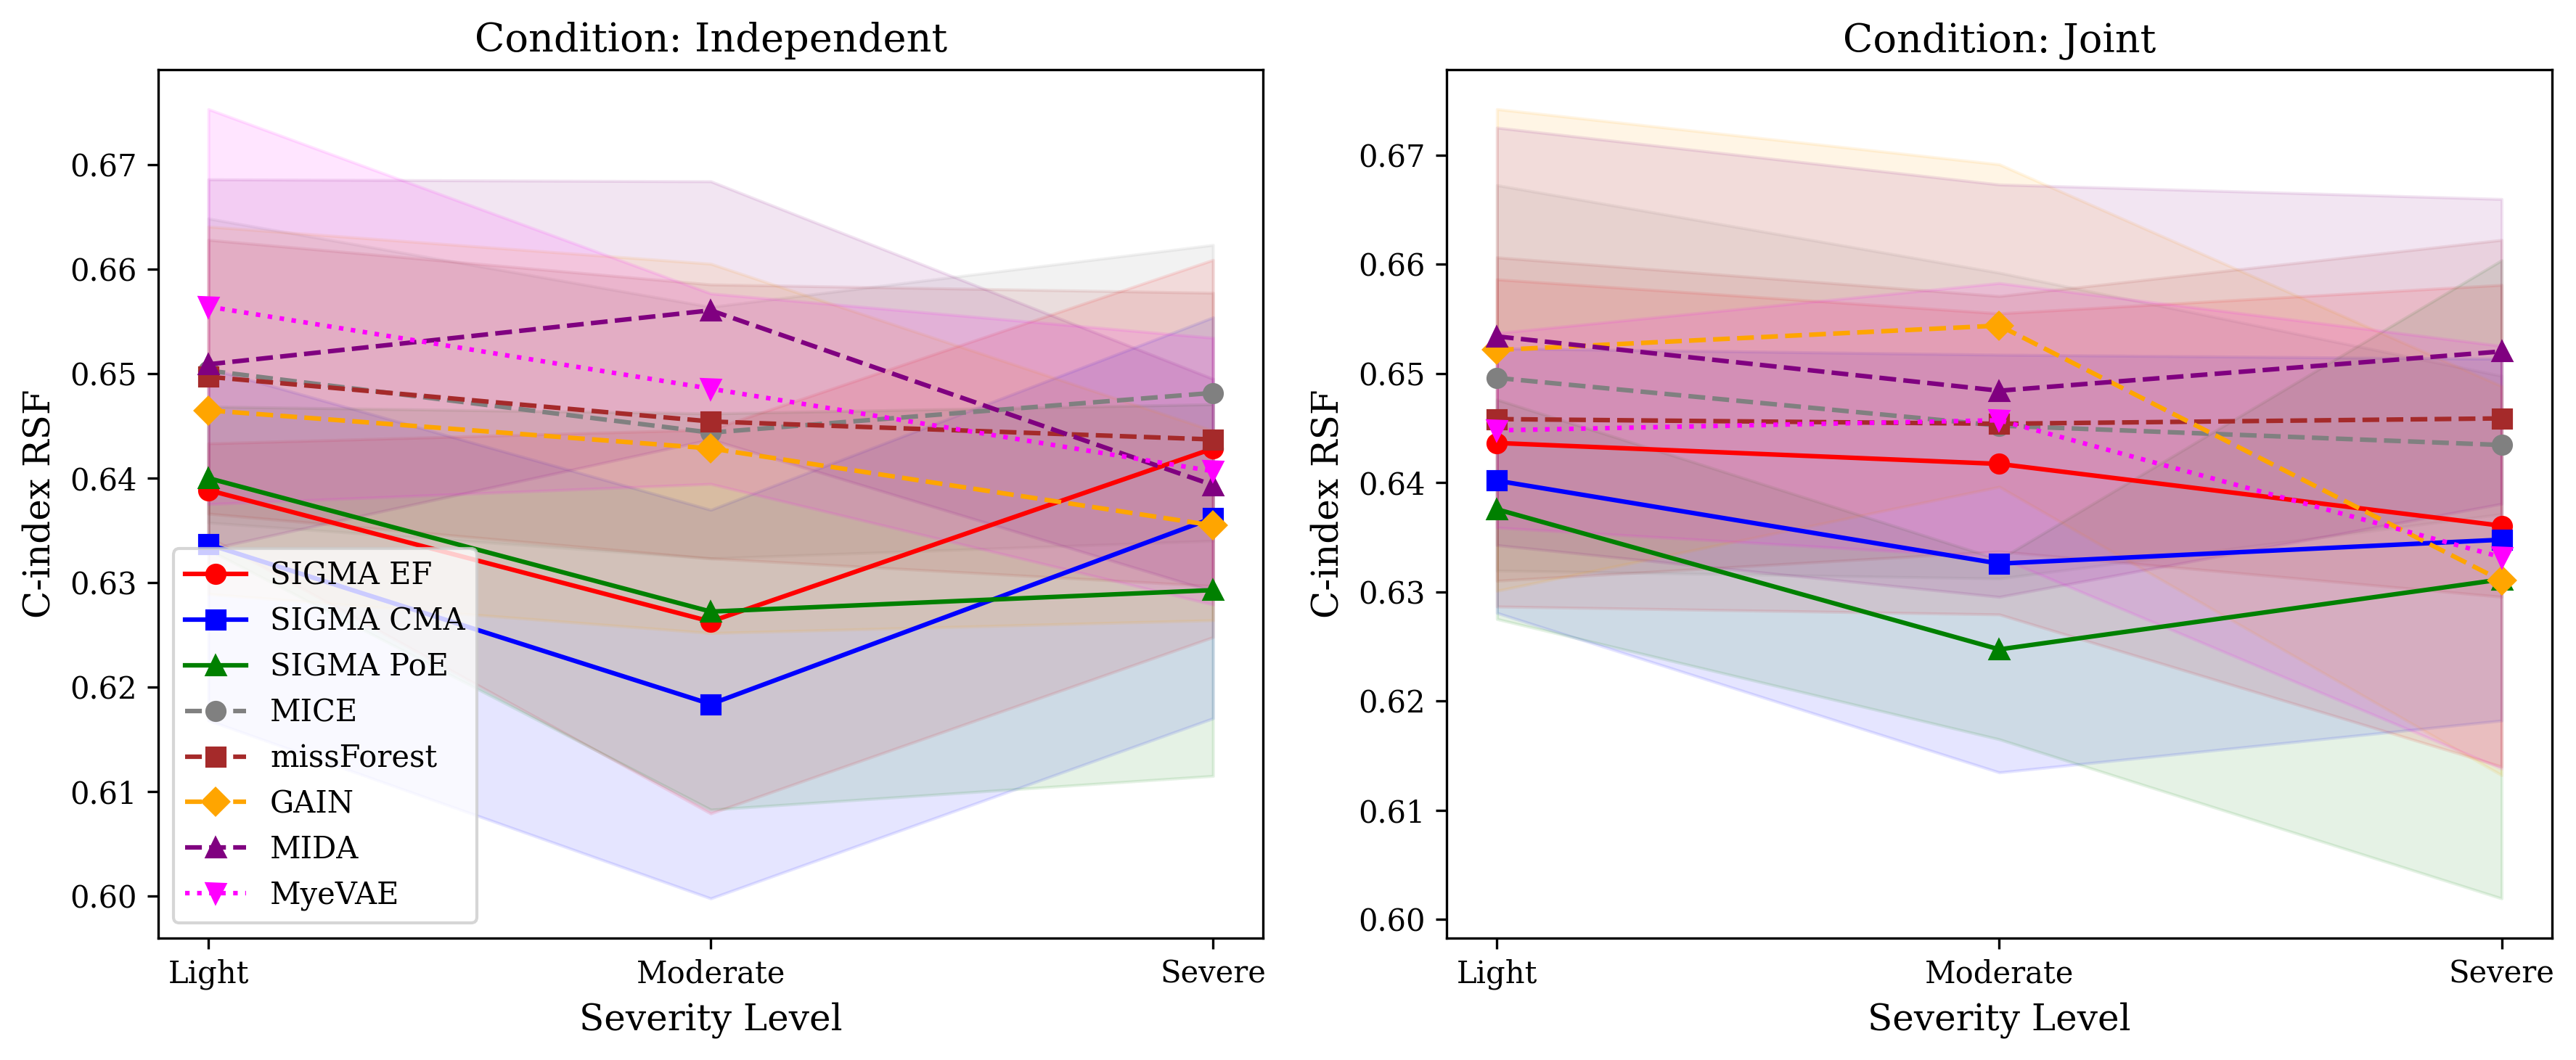
\includegraphics[width=\textwidth]{cindex_by_severity.png}
\caption{Downstream random survival forest C-index across missingness severity levels for all evaluated methods under independent (left) and joint (right) simulation conditions. Higher values indicate better survival discrimination. Error bands represent one standard deviation across five cross-validation folds.}
\label{fig:cindex_severity}
\end{figure*}

The unimodal deep learning baselines showed substantially lower survival discrimination. StandardVAE recorded C-indices of 0.634, 0.627, and 0.625 across light, moderate, and severe missingness. MNARSVAE achieved 0.636, 0.622, and 0.612 across the same levels. An ablation using only the genomic modality (SIGMA Genomic PoE) yielded a C-index of 0.500 under severe missingness, performing at chance level. These results suggest that integrating both clinical and genomic features produced substantially higher prognostic accuracy than genomic features alone.

Table~\ref{tab:direct_survival} also reports direct survival predictions from the internal Cox head of SIGMA. Under severe missingness, the internal Cox head achieved C-indices of 0.591, 0.589, and 0.604 for EF, CMA, and PoE fusion strategies, respectively, lower than the corresponding downstream RSF results. The downstream RSF outperformed the internal Cox head in survival discrimination, indicating that SIGMA functions more effectively as an imputation engine for a downstream nonlinear survival model than as a standalone survival predictor.

Table~\ref{tab:survival_ibs} reports IBS results. SIGMA and classical baselines maintained IBS values between 0.170 and 0.176 across all missingness levels. StandardVAE and MNARSVAE exhibited higher IBS values ranging from 0.188 to 0.215, indicating poorer calibration of survival probability estimates across the evaluated time horizon.



\subsection{Integration Quality and Cross-modal Imputation}

\begin{table*}[!t]
\centering
\rowcolors{2}{gray!10}{white}
\caption{CCA correlation and silhouette score across fusion strategies and severity levels.}
\label{tab:integration}
\resizebox{\columnwidth}{!}{%
\begin{tabular}{lcccccc}
\toprule
Fusion & Light CCA & Moderate CCA & Severe CCA & Light Sil & Moderate Sil & Severe Sil$^*$ \\
\midrule
EF & $0.046 \pm 0.045$ & $0.148 \pm 0.137$ & $0.080 \pm 0.105$ & $-0.011 \pm 0.005$ & $\mathbf{-0.002 \pm 0.008}$ & $-0.014 \pm 0.004$ \\
CMA & $0.276 \pm 0.096$ & $0.451 \pm 0.222$ & $0.094 \pm 0.151$ & $0.009 \pm 0.004$ & $-0.018 \pm 0.012$ & $-0.010 \pm 0.010$ \\
PoE & $\mathbf{0.795 \pm 0.142}$ & $\mathbf{0.818 \pm 0.129}$ & $\mathbf{0.597 \pm 0.190}$ & $\mathbf{0.013 \pm 0.005}$ & $-0.010 \pm 0.006$ & $\mathbf{-0.000 \pm 0.005}$ \\
MyeVAE & --- & --- & --- & $-0.008 \pm 0.009$ & $-0.025 \pm 0.004$ & $-0.041 \pm 0.006$ \\
\bottomrule
\end{tabular}%
}

\vspace{1ex}
\footnotesize{$^*$Negative silhouette scores indicate limited PAM50 subtype separation in the shared latent space. `---' indicates that MyeVAE uses concatenation without explicit cross-modal latent alignment, so CCA is not applicable.}
\end{table*}

\begin{table*}[!t]
\centering
\rowcolors{2}{gray!10}{white}
\caption{Cross-modal imputation (C2G and G2C) RMSE across fusion strategies and severity levels.}
\label{tab:crossmodal}
\resizebox{\columnwidth}{!}{%
\begin{tabular}{lcccccc}
\toprule
Fusion & Light C2G & Moderate C2G & Severe C2G & Light G2C & Moderate G2C & Severe G2C \\
\midrule
EF & $1.359 \pm 0.016$ & $1.090 \pm 0.018$ & $1.083 \pm 0.027$ & $\mathbf{1.499 \pm 0.246}$ & $\mathbf{1.747 \pm 0.249}$ & $1.291 \pm 0.195$ \\
CMA & $1.356 \pm 0.018$ & $1.159 \pm 0.058$ & $\mathbf{1.049 \pm 0.007}$ & $1.512 \pm 0.157$ & $2.582 \pm 0.932$ & $\mathbf{1.104 \pm 0.129}$ \\
PoE & $\mathbf{1.242 \pm 0.021}$ & $\mathbf{1.061 \pm 0.013}$ & $1.227 \pm 0.100$ & $---$ & $---$ & $---$ \\
\bottomrule
\end{tabular}%
}

\vspace{1ex}
\footnotesize{`---' indicates that PoE G2C cross-modal reconstruction is not reported because PoE does not support unimodal decoding; the genomic-only latent $\mathbf{z}_g$ is not trained to reconstruct clinical features independently.}
\end{table*}

Table~\ref{tab:integration} reports canonical correlation analysis (CCA) and silhouette scores across fusion strategies and missingness severity levels. The PoE fusion strategy achieved the highest CCA correlations under light ($0.795 \pm 0.142$) and moderate ($0.818 \pm 0.129$) missingness. Under severe missingness, CCA correlations decreased across all strategies, reaching $0.080 \pm 0.105$ for EF, $0.094 \pm 0.151$ for CMA, and $0.597 \pm 0.190$ for PoE. The high standard deviations observed for EF and CMA under light and severe missingness indicate variable cross-modal alignment across folds.

Silhouette scores for PAM50 subtype clustering were negative for all fusion strategies across all missingness levels, ranging from $-0.000$ to $-0.041$. Negative silhouette scores indicate that the shared latent space did not separate patients into discrete PAM50 molecular subtypes under the evaluated conditions. Figure~\ref{fig:tsne} provides a t-SNE visualization of the shared latent space under severe missingness. The lack of distinct molecular subtype clustering visually confirms the negative silhouette scores and illustrates the difficulty of unsupervised biological separation under threshold-interaction missingness.

\begin{figure*}[!t]
\centering
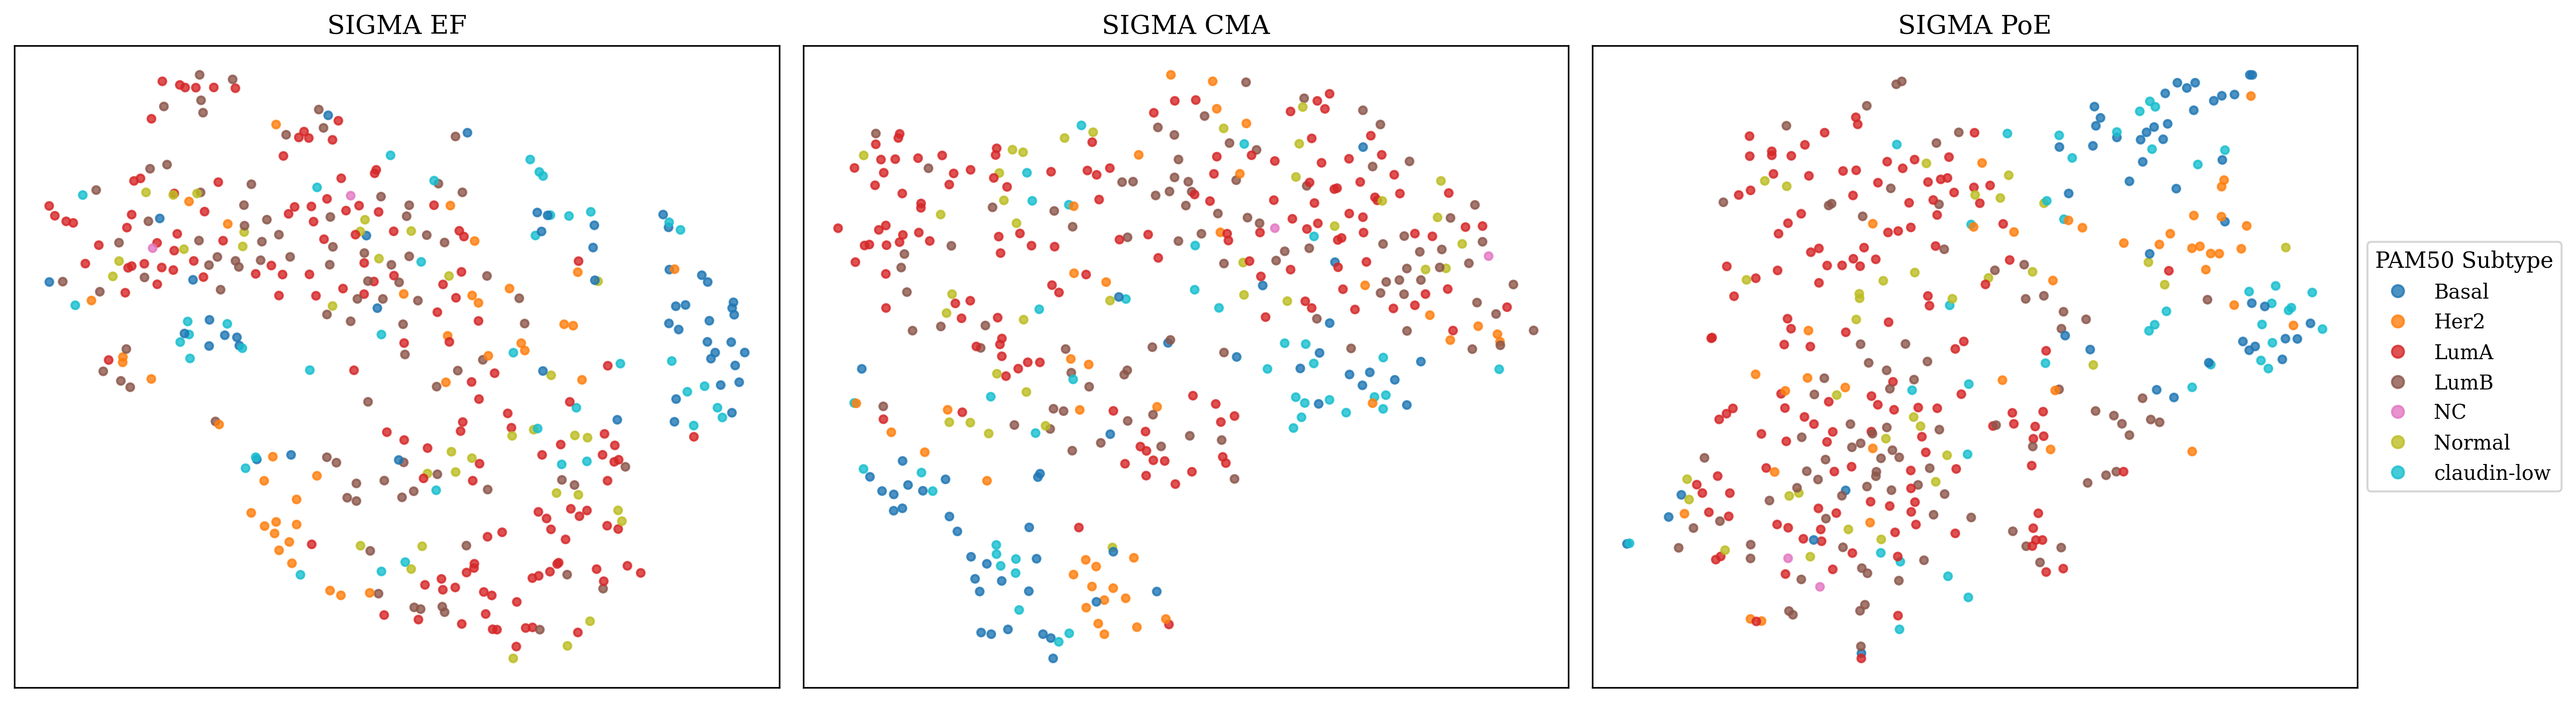
\includegraphics[width=\textwidth]{tsne_latent.png}
\caption{t-SNE visualization of the shared latent space $\mathbf{z}_{\text{shared}}$ under severe independent missingness for EF (left), CMA (center), and PoE (right) fusion strategies. Points are colored by PAM50 molecular subtype. The absence of distinct subtype clusters is consistent with the negative silhouette scores reported in Table~\ref{tab:integration}.}
\label{fig:tsne}
\end{figure*}

Table~\ref{tab:crossmodal} reports cross-modal imputation performance measured as RMSE for clinical-to-genomic (C2G) and genomic-to-clinical (G2C) directions. CMA achieved the lowest C2G RMSE across all severity levels, recording $1.049$ under severe missingness compared to $1.083$ for EF. PoE G2C RMSE is not reported because PoE does not support unimodal cross-modal reconstruction by design.



\subsection{Biological Validity}

\begin{table*}[!t]
\centering
\rowcolors{2}{gray!10}{white}
\caption{PAM50 molecular subtype classification accuracy and F1 score across all methods (severe missingness only).}
\label{tab:pam50}
\resizebox{\textwidth}{!}{%
\begin{tabular}{lccccccccc}
\toprule
Metric & SIGMA EF & SIGMA CMA & SIGMA PoE & MyeVAE & StandardVAE & MICE & missForest & GAIN & MIDA \\
\midrule
Accuracy & $0.628 \pm 0.027$ & $0.648 \pm 0.035$ & $0.625 \pm 0.036$ & $0.594 \pm 0.026$ & $0.589 \pm 0.035$ & $\mathbf{0.676 \pm 0.026}$ & $\mathbf{0.676 \pm 0.018}$ & $0.607 \pm 0.029$ & $0.632 \pm 0.025$ \\
F1 Score & $0.553 \pm 0.035$ & $0.600 \pm 0.050$ & $0.561 \pm 0.038$ & $0.524 \pm 0.041$ & $0.520 \pm 0.047$ & $0.632 \pm 0.029$ & $\mathbf{0.635 \pm 0.031}$ & $0.547 \pm 0.038$ & $0.585 \pm 0.034$ \\
\bottomrule
\end{tabular}%
}

\vspace{1ex}
\footnotesize{Note: Values are reported as mean $\pm$ standard deviation (SD) across 5 cross-validation folds. Best values are highlighted in bold. Random forest classifiers were trained on ground-truth expression values and evaluated on imputed PAM50 expression profiles under severe missingness. EF: Early Fusion; CMA: Cross-modal Attention; PoE: Product of Experts; MICE: Multiple Imputation by Chained Equations; MIDA: Missing Data Imputation using Autoencoders; GAIN: Generative Adversarial Imputation Networks; VAE: Variational Autoencoder.}
\end{table*}

Table~\ref{tab:pam50} reports PAM50 molecular subtype classification accuracy and macro F1 scores under severe missingness.

Among the evaluated imputation methods, MICE and missForest achieved the highest classification accuracy at $0.676 \pm 0.026$ and $0.676 \pm 0.018$, respectively. SIGMA CMA achieved the highest accuracy among multimodal architectures at $0.648 \pm 0.035$, outperforming MIDA ($0.632 \pm 0.025$), SIGMA EF ($0.628 \pm 0.027$), SIGMA PoE ($0.625 \pm 0.036$), and GAIN ($0.607 \pm 0.029$). Unimodal autoencoder baselines yielded the lowest classification performance, with MyeVAE recording $0.594 \pm 0.026$ and StandardVAE achieving $0.589 \pm 0.035$.

Figure~\ref{fig:pam50} compares the PAM50 molecular subtype classification accuracy across imputation methods under severe missingness. The bar chart shows that MICE and missForest achieved the two highest classification accuracies among all evaluated methods.
\begin{figure*}[!t]
\centering
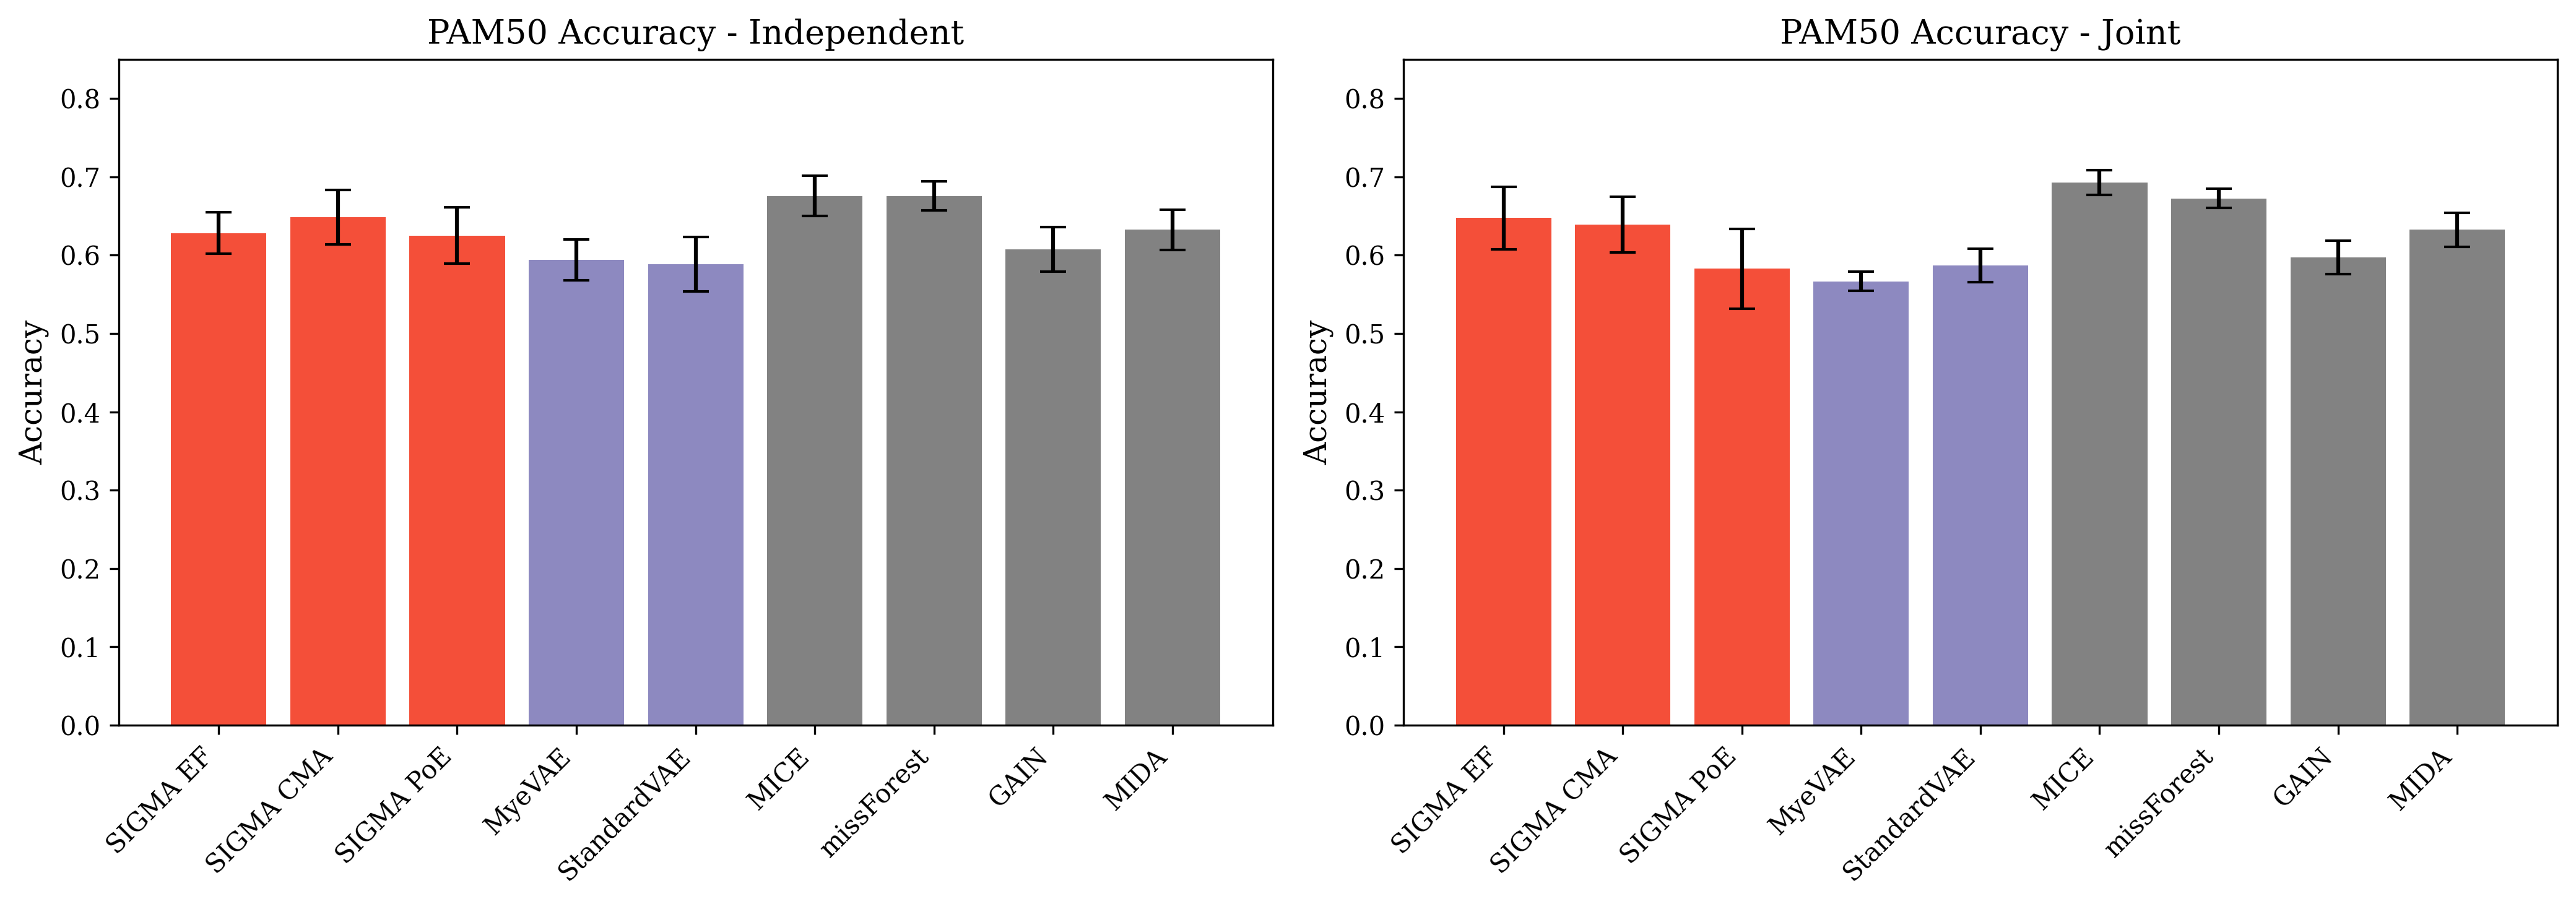
\includegraphics[width=0.8\textwidth]{pam50_accuracy.png}
\caption{PAM50 molecular subtype classification accuracy under severe missingness for all evaluated methods. Error bars represent one standard deviation across five cross-validation folds.}
\label{fig:pam50}
\end{figure*}


\section{Discussion}
\label{sec:discussion}

\subsection{Imputation Performance Under MNAR Conditions}
The results show that the imputation advantage of SIGMA EF over baseline methods expanded as the missingness severity increased, specifically within the genomic modality. Under light missingness, the genomic RMSE difference between SIGMA EF ($1.145 \pm 0.023$) and missForest ($1.065 \pm 0.019$) favored the classical baseline. Under severe missingness, SIGMA EF achieved a genomic RMSE of $0.929 \pm 0.013$, compared to missForest ($0.887 \pm 0.014$). The performance gap between the multimodal integration model and the unimodal baselines widened as the missingness rate increased.

The superior performance of Early Fusion (EF) compared to Product of Experts (PoE) contradicts the initial theoretical expectation. Prior literature proposed that PoE dynamically weights modalities based on precision, which theoretically minimizes the influence of heavily missing data streams \citep{wu2018multimodal}. In this evaluation, SIGMA EF consistently outperformed SIGMA PoE across survival metrics and imputation accuracy. Under severe missingness, SIGMA EF produced a downstream RSF C-index of $0.643 \pm 0.018$, whereas SIGMA PoE yielded $0.629 \pm 0.018$. SIGMA EF outperformed SIGMA PoE across imputation and survival metrics under all evaluated missingness conditions.

\subsection{Survival Prediction and Downstream Utility}
A performance gap separated the internal Cox survival network from the downstream random survival forest models. Under severe missingness, the internal Cox head achieved C-indices of $0.591$, $0.589$, and $0.604$ for the EF, CMA, and PoE architectures, respectively. The downstream RSF model trained on SIGMA EF imputed features achieved a C-index of $0.643 \pm 0.018$. The higher survival discrimination of the downstream RSF indicates that SIGMA functions more effectively as a multimodal feature imputation engine than as a standalone prognostic predictor.

\subsection{Biological Validity}
Despite the structural advantages of multimodal deep learning, the non-parametric missForest baseline remained highly competitive on downstream biological validation and raw imputation tasks. Under severe missingness, missForest achieved a PAM50 classification accuracy of $0.676 \pm 0.018$, with MICE achieving $0.676 \pm 0.026$ and SIGMA CMA achieving $0.648 \pm 0.035$. Furthermore, missForest yielded a genomic RMSE of $0.887 \pm 0.014$ under severe missingness, compared to SIGMA EF ($0.929 \pm 0.013$). The competitive performance of missForest indicates that classical iterative imputation methods remain strong alternatives for biological data imputation tasks.

\subsection{Integration Quality and Latent Space Analysis}
The evaluation of latent integration quality revealed limitations in preserving discrete biological structure. Silhouette scores for PAM50 subtype clustering were negative across all fusion strategies and missingness levels, with SIGMA EF recording $-0.014 \pm 0.004$ under severe missingness. Furthermore, PoE does not support unimodal cross-modal decoding by design, and its shared latent space exhibited lower PAM50 classification accuracy ($0.625 \pm 0.036$) compared to CMA ($0.648 \pm 0.035$) and classical baselines.

\subsection{Limitations}
This study is constrained by several limitations. The evaluation was restricted to the METABRIC cohort ($N=1{,}979$), limiting generalizability to larger multi-omics datasets. The TCGA cohort was used for genomic-only external validation due to the absence of paired clinical variables matching the METABRIC feature set. Model performance was evaluated using 5-fold cross-validation; the limited number of folds ($n=5$) precluded formal statistical significance testing, as the minimum achievable p-value under a two-sided Wilcoxon signed-rank test is $p=0.0625$, which exceeds the standard $\alpha=0.05$ threshold \citep{conover1999practical}.

\subsection{Future Work}
Future research will prioritize scaling multimodal imputation models to larger multi-omics repositories. Subsequent architectures may incorporate direct supervised biological regularization within the loss objective, which may improve latent subtype separation. Replacing the linear internal Cox proportional hazards head with a non-linear neural survival component could narrow the prognostic performance gap between the internal predictor and downstream tree-based survival algorithms.

\section{Conclusion}
\label{sec:conclusion}
This paper presents Survival Integration via Generative Multi-omics Alignment (SIGMA), a multimodal variational autoencoder that addresses threshold-interaction MNAR missingness across heterogeneous clinical and genomic modalities. Prior to this study, no multi-omics survival model had explicitly modeled joint threshold-interaction MNAR missingness across heterogeneous data types. Under severe missingness, the Early Fusion strategy achieved competitive genomic imputation accuracy among generative multimodal methods and maintained strong downstream survival discrimination. The evaluation showed that simple feature-level concatenation outperformed precision-weighted Product of Experts, which exhibited instability consistent with posterior collapse under severe conditions. Classical iterative imputation methods remained competitive on PAM50 biological validity classification, indicating that deep generative multimodal integration provides the primary advantage in genomic feature recovery under severe MNAR conditions.

% ============================================================
% FIGURE PLAN — to be generated after final results are complete
% ============================================================
%
% Figure 1: SIGMA Architecture Diagram
%   - Show encoder (clinical + genomic), fusion module (EF/CMA/PoE),
%     shared latent space, decoder (clinical + genomic), survival head
%   - Three panels: one per fusion strategy
%   - File: figures/sigma_architecture.pdf
%
% Figure 3: DONE - rmse_by_severity.png
% Figure 4: DONE - pam50_accuracy.png  
% Figure 5: DONE - tsne_latent.png
% Figure 6: DONE - cindex_by_severity.png
%
% ============================================================

\renewcommand{\bibfont}{\small}
\appendix
\renewcommand{\thetable}{A.\arabic{table}}
\renewcommand{\theHtable}{appendix.\arabic{table}}
\setcounter{table}{0}
\section{Supplementary Results}
\label{app:mae}

This appendix reports mean absolute error (MAE) for genomic expression imputation (Table~\ref{tab:supp_mae_g}) and clinical feature imputation (Table~\ref{tab:supp_mae_c}) across all methods and severity levels under the independent condition.

\begin{table*}[!t]
\centering
\rowcolors{2}{gray!10}{white}
\caption{MAE for genomic expression imputation across all methods and severity levels (independent condition).}
\label{tab:supp_mae_g}
\begin{tabular}{lccc}
\toprule
Method & Light (20.31\%) & Moderate (40.14\%) & Severe (59.36\%) \\
\midrule
SIGMA EF & $0.908 \pm 0.021$ & $0.833 \pm 0.016$ & $0.713 \pm 0.013$ \\
SIGMA CMA & $0.931 \pm 0.011$ & $0.854 \pm 0.013$ & $0.691 \pm 0.010$ \\
SIGMA PoE & $0.998 \pm 0.022$ & $0.856 \pm 0.012$ & $0.702 \pm 0.011$ \\
MyeVAE & $0.998 \pm 0.017$ & $0.849 \pm 0.017$ & $0.730 \pm 0.007$ \\
MICE & $0.898 \pm 0.026$ & $\mathbf{0.814 \pm 0.015}$ & $0.680 \pm 0.011$ \\
missForest & $\mathbf{0.801 \pm 0.018}$ & $0.818 \pm 0.013$ & $\mathbf{0.660 \pm 0.013}$ \\
GAIN & $1.069 \pm 0.018$ & $0.901 \pm 0.014$ & $0.797 \pm 0.007$ \\
MIDA & $0.995 \pm 0.022$ & $0.850 \pm 0.016$ & $0.714 \pm 0.010$ \\
\bottomrule
\end{tabular}

\vspace{1ex}
\footnotesize{Note: Values are reported as mean $\pm$ standard deviation (SD). Best values are highlighted in bold. MAE: Mean Absolute Error; EF: Early Fusion; CMA: Cross-modal Attention; PoE: Product of Experts; MICE: Multiple Imputation by Chained Equations.}
\end{table*}

\begin{table*}[!t]
\centering
\rowcolors{2}{gray!10}{white}
\caption{MAE for clinical feature imputation across all methods and severity levels (independent condition).}
\label{tab:supp_mae_c}
\begin{tabular}{lccc}
\toprule
Method & Light (19.91\%) & Moderate (39.80\%) & Severe (59.78\%) \\
\midrule
SIGMA EF & $0.663 \pm 0.032$ & $0.638 \pm 0.038$ & $0.471 \pm 0.022$ \\
SIGMA CMA & $0.549 \pm 0.021$ & $0.700 \pm 0.027$ & $0.449 \pm 0.028$ \\
SIGMA PoE & $0.631 \pm 0.035$ & $0.689 \pm 0.022$ & $0.428 \pm 0.019$ \\
MyeVAE & $0.615 \pm 0.027$ & $0.625 \pm 0.010$ & $0.456 \pm 0.009$ \\
MICE & $0.488 \pm 0.028$ & $0.484 \pm 0.013$ & $0.391 \pm 0.013$ \\
missForest & $\mathbf{0.382 \pm 0.022}$ & $\mathbf{0.439 \pm 0.017}$ & $\mathbf{0.323 \pm 0.019}$ \\
GAIN & $0.598 \pm 0.019$ & $0.650 \pm 0.008$ & $0.508 \pm 0.008$ \\
MIDA & $0.722 \pm 0.010$ & $0.655 \pm 0.010$ & $0.516 \pm 0.010$ \\
StandardVAE & $0.651 \pm 0.011$ & $0.598 \pm 0.008$ & $0.502 \pm 0.010$ \\
MNARSVAE & $0.736 \pm 0.066$ & $0.702 \pm 0.019$ & $0.545 \pm 0.010$ \\
\bottomrule
\end{tabular}

\vspace{1ex}
\footnotesize{Note: Values are reported as mean $\pm$ standard deviation (SD). Best values are highlighted in bold. MAE: Mean Absolute Error; EF: Early Fusion; CMA: Cross-modal Attention; PoE: Product of Experts; MICE: Multiple Imputation by Chained Equations; VAE: Variational Autoencoder; MNAR: Missing Not At Random.}
\end{table*}

\appendix
\section{Implementation and Hyperparameter Details}
\label{app:hyperparams}

All deep learning methods were implemented in PyTorch and trained on an NVIDIA RTX PRO 6000 Blackwell GPU. Hyperparameter optimization used Optuna with TPE sampling and median pruning. Tuning ran for 50 trials on fold 0 validation set only; the selected hyperparameters were then applied uniformly across all five folds. Classical baselines (MICE, missForest) used 5 trials. The composite objective for deep learning methods was $\mathcal{L}_{\text{val}} - 2.0 \times \text{C-index}_{\text{val}}$; classical baselines minimized validation RMSE only.

\begin{table*}[!ht]
\centering
\caption{Hyperparameter search spaces and fixed settings for all evaluated methods.}
\label{tab:hyperparams}
\resizebox{0.92\textwidth}{!}{%
\begin{tabular}{lll}
\toprule
Method & Tuned Hyperparameter (Search Space) & Fixed Settings / Architecture \\
\midrule
\multirow{4}{*}{SIGMA (EF, CMA, PoE)} 
  & Latent dimension $d \in \{32, 64, 128\}$ & Adam optimizer, batch size 128 \\
  & Learning rate $\in [10^{-4}, 10^{-2}]$ (log-uniform) & Max epochs 200, patience 20 \\
  & $\lambda_{\text{KL}} \in [0.01, 2.0]$, $\lambda_{\text{Cox}} \in [0.1, 5.0]$ (log-uniform) & Two-layer MLP encoders/decoders \\
  & $\lambda_{\text{cross}} \in [0.1, 1.0]$, $\kappa \in [0.05, 0.5]$ (log-uniform) & Single-head attention (CMA) \\
\midrule
\multirow{2}{*}{MyeVAE} 
  & Latent dimension $d \in \{32, 64, 128\}$; Learning rate $\in [10^{-4}, 10^{-2}]$ & Adam optimizer, batch size 128 \\
  & $\lambda_{\text{KL}} \in [0.01, 2.0]$; $\lambda_{\text{Cox}} \in [0.1, 5.0]$ (log-uniform) & Two-layer MLP encoders/decoders \\
\midrule
\multirow{2}{*}{MNARSVAE / StandardVAE} 
  & Latent dimension $d \in \{32, 64, 128\}$; Learning rate $\in [10^{-4}, 10^{-2}]$ & Adam optimizer, batch size 128 \\
  & $\lambda_{\text{KL}} \in [0.01, 2.0]$; $\lambda_{\text{Cox}} \in [0.1, 5.0]$ (log-uniform) & Clinical modality only \\
\midrule
\multirow{2}{*}{GAIN} 
  & Learning rate $\in [10^{-4}, 10^{-2}]$; Hidden dimension $\in [32, 128]$ & Adam optimizer \\
  & $\alpha \in [10, 200]$; Hint rate $\in [0.5, 0.95]$; Iterations $\in [1000, 5000]$ & Standard GAIN architecture \\
\midrule
MIDA 
  & Learning rate $\in [10^{-4}, 10^{-2}]$; Latent dim offset $\in [5, 20]$; Epochs $\in [50, 150]$ & Adam optimizer \\
\midrule
MICE 
  & \texttt{max\_iter} $\in [5, 20]$ (integer) & \texttt{n\_nearest\_features=10}, BayesianRidge \\
\midrule
missForest 
  & \texttt{n\_estimators} $\in [50, 100]$; \texttt{max\_depth} $\in \{5, 10, 20\}$; \texttt{max\_iter} $\in [5, 10]$ & Non-parametric random forest \\
\midrule
Downstream models 
  & RSF, XGBoost, DeepSurv, DeepHit & Package defaults \\
\midrule
\multirow{3}{*}{SIGMA Ablation Variants}
  & Latent dimension $d \in \{32, 64, 128\}$; Learning rate $\in [10^{-4}, 10^{-2}]$ & 50 trials per variant on fold 0 \\
  & $\lambda_{\text{KL}} \in [0.01, 2.0]$, $\lambda_{\text{Cox}} \in [0.1, 5.0]$, $\lambda_{\text{cross}} \in [0.1, 1.0]$ & $\lambda=0$ when component ablated \\
  & $\kappa \in [0.05, 0.5]$ (log-uniform) & Severe independent condition \\
\midrule
\multirow{6}{*}{Optimization Protocol}
  & Tuner & Optuna TPE + Median Pruning \\
  & Tuning trials (deep learning \& ablations) & 50 trials on fold 0 only \\
  & Tuning trials (classical) & 5 trials on fold 0 only \\
  & Tuning objective (deep learning) & $\mathcal{L}_{\text{recon}} - 2.0 \times \text{C-index}_{\text{val}}$ \\
  & Tuning objective (classical) & Validation RMSE \\
  & Cross-validation & 5-fold, best params applied to all folds \\
\bottomrule
\end{tabular}%
}

\vspace{1ex}
\footnotesize{Note: Hyperparameter tuning was performed using Tree-structured Parzen Estimator (TPE) sampling with median pruning in Optuna. The best configuration identified on fold 0 validation data was evaluated across all five cross-validation folds. EF: Early Fusion; CMA: Cross-modal Attention; PoE: Product of Experts; MICE: Multiple Imputation by Chained Equations; MIDA: Missing Data Imputation using Autoencoders; GAIN: Generative Adversarial Imputation Networks; VAE: Variational Autoencoder; MLP: Multilayer Perceptron; RSF: Random Survival Forest; TPE: Tree-structured Parzen Estimator; KL: Kullback--Leibler.}
\end{table*}

\bibliographystyle{elsarticle-harv} 
\bibliography{references}

\end{document}
